
\documentclass[pdflatex,sn-mathphys-num]{sn-jnl}

\usepackage[T1,T5]{fontenc}
\DeclareTextCommandDefault{\k}[1]{{\fontencoding{T1}\selectfont\k{#1}}}
\usepackage[utf8]{inputenc}
\usepackage{graphicx}
\usepackage{amsmath,amssymb,amsfonts}
\usepackage{amsthm}
\usepackage{xcolor}
\usepackage{textcomp}
\usepackage{manyfoot}
\usepackage{booktabs}
\usepackage{algorithm}
\usepackage{algpseudocode}
\usepackage{tikz}
\usepackage{placeins}
\usetikzlibrary{arrows.meta,calc,positioning,backgrounds}

\theoremstyle{thmstyleone}
\newtheorem{theorem}{Định lý}
\newtheorem{lemma}[theorem]{Bổ đề}
\newtheorem{proposition}[theorem]{Mệnh đề}
\newtheorem{corollary}[theorem]{Hệ quả}
\theoremstyle{thmstyletwo}
\newtheorem{example}{Ví dụ}
\newtheorem{remark}{Nhận xét}
\theoremstyle{thmstylethree}
\newtheorem{definition}{Định nghĩa}

\renewcommand{\proofname}{Chứng minh}
\renewcommand{\abstractname}{Tóm tắt}
\renewcommand{\refname}{Tài liệu tham khảo}
\renewcommand{\figurename}{Hình}
\renewcommand{\tablename}{Bảng}
\floatname{algorithm}{Thuật toán}
\algrenewcommand\algorithmicwhile{\textbf{khi}}
\algrenewcommand\algorithmicdo{\textbf{làm}}
\algrenewcommand\algorithmicif{\textbf{nếu}}
\algrenewcommand\algorithmicthen{\textbf{thì}}
\algrenewcommand\algorithmicend{\textbf{hết}}
\algrenewcommand\algorithmicreturn{\textbf{trả về}}

\newcommand{\N}{\mathbb{N}}
\newcommand{\Z}{\mathbb{Z}}
\newcommand{\cE}{\mathcal{E}}
\newcommand{\cB}{\mathcal{B}}
\newcommand{\e}{\mathbf{e}}
\newcommand{\out}{\mathrm{out}}
\newcommand{\inn}{\mathrm{in}}
\newcommand{\IN}{\mathrm{IN}}
\newcommand{\OUT}{\mathrm{OUT}}
\newcommand{\FIX}{\textup{\textsc{Fix}}}
\newcommand{\FREE}{\textup{\textsc{Free}}}
\newcommand{\SFIX}{\textup{\textsc{Strict-Fix}}}
\newcommand{\SFREE}{\textup{\textsc{Strict-Free}}}
\newcommand{\abs}[1]{\lvert #1\rvert}
\newcommand{\floor}[1]{\lfloor #1\rfloor}
\newcommand{\YES}{\texttt{YES}}
\newcommand{\NO}{\texttt{NO}}

\definecolor{cA}{HTML}{0072B2}
\definecolor{cB}{HTML}{D55E00}
\definecolor{cTa}{HTML}{009E73}
\definecolor{cTb}{HTML}{E69F00}
\tikzset{
  >={Stealth[length=4.5pt,width=3.6pt]},
  vtx/.style={circle,draw,semithick,fill=white,minimum size=5.6mm,inner sep=0pt,font=\small},
  svtx/.style={circle,draw,semithick,fill=white,minimum size=5.4mm,inner sep=0pt,font=\footnotesize},
  port/.style={circle,draw,semithick,fill=white,minimum size=2.4mm,inner sep=0pt},
  tlab/.style={fill=white,inner sep=1pt,font=\scriptsize,text=black},
  cnt/.style={rectangle,rounded corners=1pt,draw,thin,fill=white,inner sep=1.5pt,font=\scriptsize},
  sub/.style={font=\footnotesize},
  note/.style={font=\scriptsize,text=black!70,align=left},
  t1/.style={cTa,very thick},
  t2/.style={cTb,very thick,densely dashed},
  walkA/.style={cA,very thick,->},
  walkB/.style={cB,very thick,->,densely dashed},
}
\raggedbottom

\begin{document}

\title[Phủ chính xác cạnh bằng walk thời gian]{Phủ chính xác cạnh bằng walk thời gian chặt và không chặt}

\author[1]{\fnm{Duc Thien} \sur{Quach}}\email{23020161@vnu.edu.vn}

\author*[1]{\fnm{Manh Cuong} \sur{Tran}}\email{tranmanhcuong@vnu.edu.vn}

\affil[1]{\orgdiv{Faculty of Information Technology}, \orgname{VNU University of Engineering and Technology}, \orgaddress{\city{Hanoi}, \country{Vietnam}}}

\abstract{Bài toán phủ chính xác cạnh hỏi liệu các cạnh của một đồ thị thời gian có $n$ đỉnh và $m$ cạnh có thể được phân hoạch thành các walk tuân theo nhãn thời gian hay không, với số walk xuất phát tại mỗi đỉnh cho trước và, trong biến thể đầu cuối cố định, cả số walk kết thúc tại mỗi đỉnh. Với walk không chặt, chúng tôi chứng minh bài toán giải được trong thời gian đa thức bằng một cách tiếp cận mới dựa trên tính M-lồi, đồng thời lấp một lỗ hổng trong phác thảo chứng minh của một phép quy tĩnh trước đây. Một định hướng các cạnh thực hiện được bằng walk khi và chỉ khi các bộ đếm walk luôn không âm và mỗi thành phần snapshot chứa một walk, và chỉ những thành phần có mọi bậc và bộ đếm đều chẵn mới có thể vi phạm điều kiện sau. Sau khi bỏ trạng thái chết, tập trạng thái của mỗi thành phần như vậy là M-lồi. Từ đó ta có thuật toán đường tăng trả về các walk hoặc một chứng nhận vô nghiệm, dùng nhiều nhất $m/2$ lần tăng và $O(n+nm^2)$ phép toán số học khi định hướng lại bằng đảo đường. Bản cài đặt đã được kiểm chứng trên các instance nhỏ. Với walk chặt, chúng tôi chứng minh bài toán là NP-đầy đủ, ngay cả khi chỉ có sáu nhãn thời gian với đầu cuối cố định và hai nhãn với đầu cuối tự do.}

\keywords{Đồ thị thời gian, Phủ chính xác cạnh, Walk thời gian, Tập M-lồi, Luồng submodular, NP-đầy đủ}

\pacs[MSC Classification]{05C85, 90C27, 90C35, 68Q17}

\maketitle

\section{Giới thiệu}\label{sec:intro}

Đồ thị thời gian mô hình hóa các kết nối có tính sẵn có thay đổi theo thời gian~\cite{holme2012,michail2016}. Trong định tuyến cung, các cạnh biểu diễn những nhiệm vụ cần được phục vụ, trong lập lịch phương tiện, các chuyến đi theo thứ tự thời gian phải được ghép thành các ca xe~\cite{edmonds1973,corberan2015,bunte2009}. Những bối cảnh này thúc đẩy việc phủ cạnh bằng các walk tuân theo nhãn thời gian. Chúng tôi xét các cạnh vô hướng, nên chiều đi qua mỗi nhiệm vụ hoặc tiếp xúc được chọn đồng thời với các walk. Đóng góp của chúng tôi thuộc về cấu trúc và thuật toán, các thực nghiệm, vốn bỏ qua hướng được ghi nhận và thời gian di chuyển, kiểm tra tính đúng đắn và khả năng mở rộng chứ không mô hình hóa một ứng dụng định tuyến.

Một phủ chính xác cạnh phân hoạch mọi cạnh thời gian thành các walk: đi qua mỗi cạnh đúng một lần. Đầu vào cho trước số walk xuất phát tại mỗi đỉnh. Trong \FIX{}, đầu vào cũng cho trước số walk kết thúc tại mỗi đỉnh, không ghép cặp từng đỉnh xuất phát và kết thúc, trong \FREE{}, lời giải chọn các đỉnh kết thúc. Walk rỗng được cho phép. Một walk không chặt dùng các nhãn thời gian không giảm và có thể đi qua nhiều cạnh của một snapshot (các cạnh có cùng nhãn thời gian), còn một walk chặt dùng các nhãn thời gian tăng nghiêm ngặt và nhiều nhất một cạnh trong mỗi snapshot. Các dấu thời gian bằng nhau xuất hiện tự nhiên trong dữ liệu tiếp xúc được ghi với độ phân giải thô. Sự phân biệt giữa đi qua cạnh chặt và không chặt có thể làm thay đổi độ phức tạp~\cite{casteigts2024,erlebach2023}, kể cả trong bài toán thăm dò theo thời gian. 

Deligkas và cộng sự~\cite{deligkas2025} giới thiệu bài toán phủ chính xác cạnh thời gian tại AAAI 2025, đặt ra bài toán và đưa ra các kết quả về độ phức tạp. Bài báo này phát triển từ bài toán và ký hiệu của họ. Họ khẳng định walk không chặt giải được trong thời gian đa thức thông qua một phép quy tĩnh. Kết quả NP-đầy đủ của họ khi không cho trước đỉnh xuất phát liên quan đến việc cực tiểu hóa số walk, còn trường hợp chặt với đầu cuối cho trước được để mở. Phép quy tĩnh trong phác thảo chứng minh Định lý~6.3 của họ bỏ sót một điều kiện về tính sẵn có theo thời gian: mọi thành phần liên thông của một snapshot có chứa cạnh phải chứa một walk ngay trước thời điểm của nó. Liên thông tĩnh tới một đầu cuối không bảo đảm điều này. Mục~\ref{sec:counterexample} đưa ra một instance năm đỉnh mà đồ thị tĩnh có một phủ chính xác cạnh mặc dù đồ thị thời gian không có, theo phép dựng đầu cuối kết thúc ở Hình~3 của~\cite{deligkas2025} (cách hiểu của chúng tôi). Lỗ hổng này không bác bỏ khẳng định của họ. Chúng tôi xác lập kết quả đa thức cho trường hợp không chặt bằng một lập luận khác và giải quyết các biến thể chặt.

Phương pháp của chúng tôi đặc trưng các định hướng khả thực hiện bằng số walk không âm và sự hiện diện của một walk trong mỗi thành phần snapshot. Chỉ các thành phần có bậc và bộ đếm chẵn mới có thể vi phạm điều kiện sau. Đếm theo cặp làm lộ ra các trạng thái thành phần M-lồi, và việc bỏ trạng thái chết vẫn bảo toàn tính M-lồi. Điều này dẫn đến một mô hình giao M-lồi và một thuật toán đường tăng sửa các thành phần chết hoặc chứng nhận vô nghiệm. Theo hiểu biết của chúng tôi, cách xử lý trạng thái chết là mới.

\paragraph{Đóng góp.}
\begin{enumerate}
\item \emph{Đặc trưng và lỗ hổng.} Một định hướng khả thực hiện khi và chỉ khi điều kiện đếm được thỏa mãn và mỗi thành phần snapshot chứa một walk (Định lý~\ref{thm:char}), chỉ thành phần chẵn mới có thể vi phạm điều kiện sau (Bổ đề~\ref{lem:noneven}), và instance không có thành phần như vậy quy về một luồng cực đại (Hệ quả~\ref{cor:flow}). Theo phép dựng đầu cuối kết thúc thể hiện ở Hình~3 của~\cite{deligkas2025}, một instance năm đỉnh cho thấy lỗ hổng trong phép quy tĩnh (Mệnh đề~\ref{prop:aaai}, Bổ đề~\ref{lem:aaai}).
\item \emph{Thuật toán khả thi M-lồi.} Chúng tôi chứng minh việc bỏ trạng thái chết vẫn bảo toàn tính M-lồi của trạng thái thành phần chẵn (Bổ đề~\ref{lem:gamma}(b)), từ đó thu được thuật toán đa thức thông qua tính khả thi của một giao M-lồi (Định lý~\ref{thm:reduction}). Thuật toán trả về các walk hoặc chứng nhận vô nghiệm (Định lý~\ref{thm:correct}) và có cận của Định lý~\ref{thm:time}.
\item \emph{Độ khó của walk chặt.} Bài toán chặt là NP-đầy đủ khi đầu cuối được chỉ định và có sáu nhãn thời gian, cũng như khi đầu cuối tự do và có hai nhãn thời gian, cho phép walk rỗng (Định lý~\ref{thm:strict}).
\end{enumerate}

\section{Phát biểu bài toán và công trình liên quan}\label{sec:prelim}

\subsection{Phát biểu bài toán}\label{sec:problem}

Ta ký hiệu $\N=\{0,1,2,\ldots\}$ và dùng $\Z$ cho các số nguyên. Đồ thị thời gian vô hướng là $G=(V,\cE,\tau)$, với nhãn cạnh $\tau:\cE\to\N$, $n=\abs{V}$ và $m=\abs{\cE}$. Cạnh song song là các cạnh phân biệt, khuyên bị loại trừ. Tại thời điểm $t$, $G_t=(V,E_t)$, với $E_t=\{e\in\cE:\tau(e)=t\}$, là \emph{snapshot}, thành phần snapshot chứa ít nhất một cạnh.

Một \emph{walk thời gian không chặt} là $W=(v_0,e_1,v_1,\ldots,e_\ell,v_\ell)$, trong đó $e_i$ nối $v_{i-1}$ với $v_i$ và $\tau(e_1)\le\cdots\le\tau(e_\ell)$, đỉnh đầu và cuối lần lượt là $v_0,v_\ell$. Walk rỗng có $\ell=0$. Phủ chính xác cạnh đi qua mỗi cạnh đúng một lần trên toàn bộ các walk.

Hai bài toán quyết định chính cho trước một vector $a\in\N^V$ gồm số lượng xuất phát, với $k=\sum_v a_v$.

\begin{definition}\label{def:problems}
\begin{itemize}
\item \FREE{}: quyết định liệu có tồn tại $k$ walk thời gian không chặt cùng nhau đi qua mỗi cạnh của $\cE$ đúng một lần, với đúng $a_v$ walk xuất phát tại mỗi đỉnh $v$, hay không.
\item \FIX{}: cho thêm một vector $z\in\N^V$, quyết định liệu có tồn tại các walk thỏa mãn \FREE{} với đúng $z_v$ walk kết thúc tại mỗi đỉnh $v$, hay không.
\end{itemize}
\end{definition}

Trong \FIX{}, $a$ và $z$ cho trước số lượng đầu mút mà không ghép cặp đỉnh xuất phát với đỉnh kết thúc. Nếu không nói khác, walk là không chặt.

Thời gian chạy đếm các phép toán số học chi phí đơn vị trên số nguyên một từ máy, gồm $a_v,z_v$. Chúng tôi trả về một lời giải \emph{nén} (các walk không rỗng và số walk rỗng tại mỗi đỉnh), vì bội số nhị phân có thể đòi hỏi liệt kê số walk rỗng tăng theo hàm mũ.

\subsection{Công trình liên quan}\label{sec:related}

\paragraph{Phủ chính xác cạnh trong đồ thị thời gian.}
Deligkas và cộng sự~\cite{deligkas2025} nghiên cứu đường đi, trail và walk thời gian (số định lý và số trang theo bản AAAI, còn bản mở rộng được trích dẫn là arXiv v1). Với walk chặt có đầu cuối cố định, Hệ quả~6.4 xét đồ thị thời gian proper (mỗi snapshot là một cặp ghép), còn Định lý~6.5 cho thuật toán $O(2^k k\,t_{\max})$ khi $|E_t|\in\{0,k\}$ ($t_{\max}$ là nhãn thời gian lớn nhất). Các trường hợp có hướng giải được trong thời gian đa thức (Định lý~6.1 và~5.2). Định lý~6.3 nhắc đến đầu cuối xuất phát, trong khi chứng minh và Hình~3 dùng đầu cuối kết thúc~\cite{deligkas2025}. Bản mở rộng~\cite{deligkas2024arxiv} nêu rõ cả hai. Mục~\ref{sec:counterexample} chỉ phân tích chi tiết phép dựng đầu cuối kết thúc thể hiện trong chứng minh và Hình~3. Biến thể chỉ có đầu cuối xuất phát không được xét ở đây.

\paragraph{Mạng thời gian và các bài toán phủ.}
Biểu diễn bản sao thời gian xuất hiện trong~\cite{akrida2019}. Marino và Silva nghiên cứu một walk đơn đi qua mỗi cạnh một lần trong đồ thị thời gian~\cite{marino2023}, với $k=1$, đỉnh xuất phát cho trước và một nhãn cho mỗi cạnh, tính khả thi không chặt quy về, theo Định lý~\ref{thm:char}, một phép kiểm tra đường đi Euler theo từng snapshot, nên chúng tôi không so sánh các kết quả độ phức tạp giữa hai mô hình. Các bài toán liên quan khác khám phá mọi cạnh~\cite{bumpus2023} hoặc phủ đỉnh của DAG thời gian~\cite{chakraborty2024}.

\paragraph{Tính lồi rời rạc và định hướng.}
Chúng tôi dùng tập M-lồi~\cite{murota1996,murota2003}, luồng submodular~\cite{edmonds1977,franktardos1988,murota2003,fujishige2005}, định hướng ràng buộc bậc~\cite{hakimi1965,frank1980,frank2011} và đường tăng~\cite{cunningham1985,fujishige2005}. Ràng buộc bổ sung của chúng tôi loại trạng thái chết của một thành phần chẵn. Cấu trúc liên quan gồm định hướng liên thông mạnh~\cite{abdi2025}.

\section{Định hướng, thành phần chẵn và lỗ hổng trong phép quy tĩnh}\label{sec:char}

\subsection{Định hướng và bộ đếm walk}

Một walk đi qua cạnh $\{u,v\}$ từ $u$ đến $v$ \emph{định hướng} nó thành $u\to v$, và $u$ được gọi là \emph{đuôi}. Một lời giải do đó cảm sinh một định hướng của mọi cạnh. Với một định hướng, gọi $\out_t(v)$ và $\inn_t(v)$ lần lượt là số cung của $E_t$ có đuôi $v$ và có đầu $v$. \emph{Bộ đếm walk} $c_t(v)$ là số walk tại $v$ ngay trước thời điểm $t$. Bộ đếm bắt đầu từ $a_v$ và tiến hóa theo
\[
  c_{t^+}(v)=c_t(v)-\out_t(v)+\inn_t(v),
\]
trong đó $t^+$ là thời điểm ngay sau $t$. Tính chẵn lẻ của bộ đếm được xác định bởi $a_v$ cộng số cạnh kề với $v$ trước $t$, không phụ thuộc vào định hướng. Một walk được tính đúng một lần tại đỉnh hiện thời, tại cùng một nhãn thời gian, walk có thể đi qua liên tiếp nhiều cạnh.

Gọi $t_{v,1}<\dots<t_{v,q_v}$ là các nhãn thời gian mà $v$ có cạnh kề (các \emph{lần xuất hiện} của $v$), gọi $g_{v,j}$ là bậc của $v$ trong $E_{t_{v,j}}$, và đặt $G_{v,j}=\sum_{i\le j}g_{v,i}$ và $G_v=G_{v,q_v}$. Với một định hướng, gọi $b_{v,j}$ là số cung của $E_{t_{v,j}}$ có đuôi $v$ và $B_{v,j}=\sum_{i\le j}b_{v,i}$, trong đó tổng rỗng bằng không. Với \FIX{}, chúng tôi đặt $h_v=(a_v+G_v-z_v)/2$, là số cung có đuôi $v$ trong mọi lời giải, được xác định bởi số walk cuối cùng $z_v$.

\begin{theorem}\label{thm:char}
Một định hướng là khả thi bởi các walk xuất phát theo $a$ (bài toán \FREE{}) khi và chỉ khi, tại mọi thời điểm $t$,
\begin{enumerate}
\item[(i)] $\out_t(v)-\inn_t(v)\le c_t(v)$ với mọi đỉnh $v$, và
\item[(ii)] mọi thành phần snapshot $K$ của $E_t$ đều chứa một walk, tức là $\sum_{v\in K}c_t(v)\ge 1$.
\end{enumerate}
Với \FIX{}, điều kiện bổ sung là số walk cuối cùng tại $v$ bằng $z_v$ với mọi $v$, tức là $B_{v,q_v}=h_v$.
\end{theorem}

\begin{proof}
\emph{Điều kiện cần.} Tại thời điểm $t$, mỗi cạnh rời khỏi $v$ hoặc là cạnh đầu tiên mà một walk dùng tại thời điểm $t$, khi đó walk đã ở $v$ trước $t$ nên có nhiều nhất $c_t(v)$ cạnh như vậy, hoặc đi sau một cạnh đi vào $v$ tại thời điểm $t$ trên cùng walk, và mỗi cạnh đi vào có nhiều nhất một cạnh kế tiếp. Do đó $\out_t(v)\le c_t(v)+\inn_t(v)$, đó là~(i). Các cạnh mà một walk dùng tại thời điểm $t$ tạo thành một đường (trail) trong một thành phần $K$ của $E_t$, và walk nằm tại đỉnh đầu tiên của đường này ngay trước $t$. Do đó mọi thành phần có cạnh đều chứa một walk. Với \FIX{}, số walk cuối cùng tại $v$ là $a_v+G_v-2B_{v,q_v}=z_v$.

\emph{Điều kiện đủ.} Ta xử lý các thời điểm theo thứ tự tăng dần và các thành phần của $E_t$ một cách độc lập. Gọi $\vec K$ là đồ thị có hướng của $K$ và $r=\sum_{v\in K}\max(0,\out_t(v)-\inn_t(v))$. Nếu $r>0$, thêm $r$ cung giả từ các đỉnh có $\inn>\out$ đến các đỉnh có $\out>\inn$, ghép mỗi đơn vị thiếu hụt với một đơn vị thặng dư. Tổng hai loại bằng nhau vì tổng $\out_t-\inn_t$ trên $K$ bằng không. Như vậy mỗi đỉnh được cân bằng. Đồ thị tăng cường liên thông yếu vì $K$ liên thông và các cung thêm nối các đỉnh của $K$, do đó nó có chu trình Euler. Theo thứ tự vòng tròn, bỏ $r$ cung giả sẽ còn đúng $r$ đường (Hình~\ref{fig:dummy}), mỗi đường bắt đầu tại đầu mút đi vào của một cung giả (một đỉnh thặng dư) và kết thúc tại đầu mút đi ra của cung giả kế tiếp. Đỉnh $v$ có thặng dư là đầu mút đi vào của đúng $\out_t(v)-\inn_t(v)$ cung giả, nên có bấy nhiêu đường bắt đầu tại đó. Theo (i), $v$ có đủ walk để đi các đường này. Nếu $r=0$ thì $\vec K$ là Euler. Theo (ii) có một đỉnh của $K$ đang giữ một walk, và walk này đi theo một chu trình Euler xuất phát từ đỉnh đó. Mọi walk khác đứng chờ. Số walk tại mỗi đỉnh sau $t$ bằng $c_{t^+}$, nên quy nạp tiếp tục. Với \FIX{}, số cuối cùng là $z$.
\end{proof}

Chứng minh điều kiện đủ cho một thuật toán $O(n+m)$, sau khi sắp xếp các cạnh, xây dựng các walk từ một định hướng thỏa mãn (i) và (ii) bằng thuật toán Hierholzer~\cite{hierholzer1873}, do đó, khi hướng của mọi cạnh được cho trước, \FREE{} và \FIX{} được quyết định trong thời gian $O(n+m\log(m+1))$.

\begin{figure}[!htb]
\centering
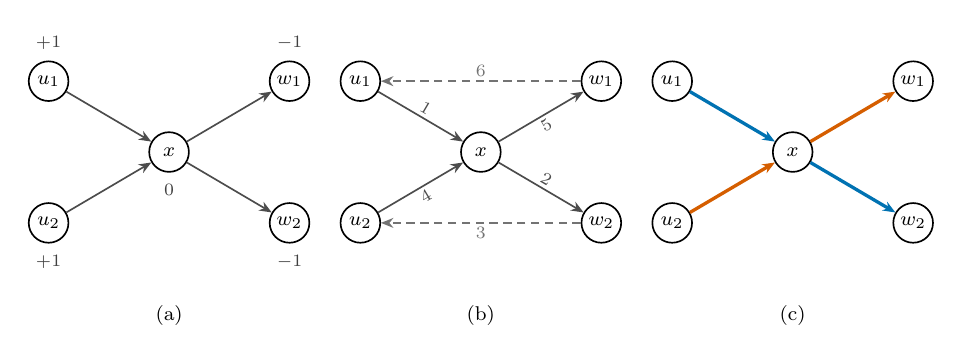
\begin{tikzpicture}[scale=0.9,transform shape,
  vx/.style={circle,draw,semithick,fill=white,minimum size=5.6mm,inner sep=0pt,font=\footnotesize},
  arc/.style={->,semithick,black!70},
  dum/.style={->,semithick,densely dashed,black!55},
  tA/.style={->,very thick,cA},
  tB/.style={->,very thick,cB},
  num/.style={font=\scriptsize,inner sep=1.5pt},
  imb/.style={font=\scriptsize,text=black!75}]
  \foreach \o/\p in {0/a,4.4/b,8.8/c} {
    \node[vx] (u1\p) at (\o,1) {$u_1$};
    \node[vx] (u2\p) at (\o,-1) {$u_2$};
    \node[vx] (x\p)  at (\o+1.7,0) {$x$};
    \node[vx] (w1\p) at (\o+3.4,1) {$w_1$};
    \node[vx] (w2\p) at (\o+3.4,-1) {$w_2$};
  }
  \draw[arc] (u1a) -- (xa);
  \draw[arc] (u2a) -- (xa);
  \draw[arc] (xa) -- (w1a);
  \draw[arc] (xa) -- (w2a);
  \node[imb,above=1pt] at (u1a.north) {$+1$};
  \node[imb,below=1pt] at (u2a.south) {$+1$};
  \node[imb,above=1pt] at (w1a.north) {$-1$};
  \node[imb,below=1pt] at (w2a.south) {$-1$};
  \node[imb,below=1pt] at (xa.south) {$0$};
  \draw[arc] (u1b) -- node[num,above,sloped] {1} (xb);
  \draw[arc] (xb) -- node[num,above,sloped] {2} (w2b);
  \draw[arc] (u2b) -- node[num,below,sloped] {4} (xb);
  \draw[arc] (xb) -- node[num,below,sloped] {5} (w1b);
  \draw[dum] (w2b) -- node[num,below] {3} (u2b);
  \draw[dum] (w1b) -- node[num,above] {6} (u1b);
  \draw[tA] (u1c) -- (xc);
  \draw[tA] (xc) -- (w2c);
  \draw[tB] (u2c) -- (xc);
  \draw[tB] (xc) -- (w1c);
  \node[font=\footnotesize] at (1.7,-2.3) {(a)};
  \node[font=\footnotesize] at (6.1,-2.3) {(b)};
  \node[font=\footnotesize] at (10.5,-2.3) {(c)};
\end{tikzpicture}
\caption{Các cung giả trong chứng minh Định lý~\ref{thm:char}, minh họa trên một thành phần có hai đỉnh thặng dư $u_1,u_2$ và hai đỉnh thiếu hụt $w_1,w_2$. (a) Thành phần có hướng, với $\out_t-\inn_t$ tại mỗi đỉnh. (b) Các cung giả nét đứt nối mỗi đỉnh thiếu hụt với một đỉnh thặng dư; các số từ 1 đến 6 biểu thị một chu trình Euler. (c) Bỏ các cung giả còn lại hai đường, từ $u_1$ đến $w_2$ và từ $u_2$ đến $w_1$.}
\label{fig:dummy}
\end{figure}

\subsection{Thành phần chẵn và mạng chuỗi}

\begin{definition}\label{def:even}
Một thành phần snapshot $K$ của $E_t$ là \emph{chẵn} nếu mọi đỉnh của $K$ có bậc chẵn trong $E_t$ và bộ đếm walk $c_t$ chẵn. Một thành phần chẵn là \emph{chết} dưới một định hướng nếu $c_t(v)=0$ với mọi $v\in K$.
\end{definition}

Hai cạnh song song và một tam giác có bộ đếm walk chẵn là các thành phần chẵn. Một đường đi không chẵn.

\begin{lemma}\label{lem:noneven}
Nếu một định hướng thỏa mãn (i) và thành phần snapshot $K$ của $E_t$ không chẵn, thì $K$ thỏa mãn (ii).
\end{lemma}

\begin{proof}
Nếu có đỉnh của $K$ có bậc lẻ trong $E_t$, thì $\out_t-\inn_t$ lẻ và do đó khác không tại đỉnh đó. Vì tổng của $\out_t-\inn_t$ bằng $0$ trên $K$, có một đỉnh với $\out_t-\inn_t>0$, và theo (i) nó có $c_t\ge1$. Nếu bộ đếm $c_t(v)$ lẻ thì đó là số nguyên lẻ không âm, và do đó ít nhất bằng một: $c_t(v)$ bằng $a_v\ge0$ tại lần xuất hiện đầu tiên của $v$ và ngược lại là bộ đếm $c_{t'^+}(v)$ sau lần xuất hiện trước đó $t'$, không âm theo~(i) tại $t'$.
\end{proof}

Điều kiện (i) yêu cầu bộ đếm walk sau lần xuất hiện thứ $j$ của $v$, tức là $a_v+G_{v,j}-2B_{v,j}$, không âm., điều này tương đương với $B_{v,j}\le\floor{(a_v+G_{v,j})/2}$.

Chúng tôi áp đặt các cận này dưới dạng sức chứa trong một \emph{mạng chuỗi} có một nguồn và một đích $r$. Với mỗi lần xuất hiện $(v,j)$ có một nút $s_{v,j}$, và các nút này tạo thành một chuỗi $s_{v,1}\to\dots\to s_{v,q_v}\to r$. Cung rời khỏi $s_{v,j}$ có sức chứa $C_{v,j}=\floor{(a_v+G_{v,j})/2}$ trong \FREE{}, và $C_{v,j}=\min(\floor{(a_v+G_{v,j})/2},h_v)$ trong \FIX{}. Với mỗi cạnh $e=\{u,v\}$ có nhãn thời gian $t$, có một nút nhận một đơn vị từ nguồn và có hai cung sức chứa $1$ tới các nút lần xuất hiện của $u$ và $v$ tại thời điểm $t$.

Đơn vị của $e$ đi tới đầu mút được chọn làm đuôi, nên luồng trên cung rời khỏi $s_{v,j}$ bằng $B_{v,j}$. Mạng có $O(m)$ nút và cung, và với \FREE{} một luồng có giá trị $m$ tương ứng chính xác với một định hướng thỏa mãn (i). Bộ đếm sau lần xuất hiện $j$ là $a_v+G_{v,j}-2B_{v,j}$, nên sức chứa trên mỗi cung chuỗi đi ra bảo đảm bộ đếm không âm.

Hình~\ref{fig:chain} minh họa $e=\{u,v\}$ rồi đến $f=\{v,w\}$: các đơn vị từ $\sigma$ chọn đuôi cạnh, và các cung chuỗi đậm có sức chứa $C_{v,j}$.

\begin{figure}[t]
\centering
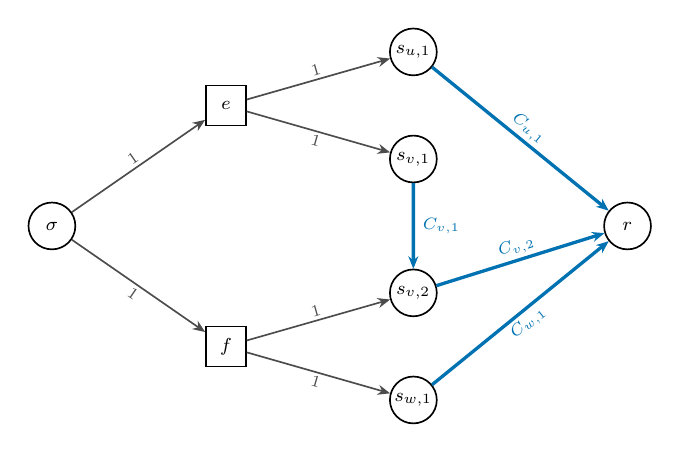
\begin{tikzpicture}[scale=0.85,transform shape,x=1cm,y=1cm,
  lbl/.style={font=\scriptsize,inner sep=1.5pt},
  occ/.style={circle,draw,semithick,fill=white,minimum size=7mm,inner sep=0pt,font=\footnotesize},
  edg/.style={rectangle,draw,semithick,fill=white,minimum size=6mm,inner sep=0pt,font=\footnotesize},
  flow/.style={->,semithick,black!70},
  chain/.style={->,very thick,cA}]
  \node[circle,draw,semithick,fill=white,minimum size=7mm,inner sep=0pt,font=\footnotesize] (src) at (0,0) {$\sigma$};
  \node[edg] (e) at (2.6,1.8) {$e$};
  \node[edg] (f) at (2.6,-1.8) {$f$};
  \node[occ] (su1) at (5.4,2.6) {$s_{u,1}$};
  \node[occ] (sv1) at (5.4,1.0) {$s_{v,1}$};
  \node[occ] (sv2) at (5.4,-1.0) {$s_{v,2}$};
  \node[occ] (sw1) at (5.4,-2.6) {$s_{w,1}$};
  \node[occ] (r) at (8.6,0) {$r$};
  \draw[flow] (src) -- node[lbl,pos=0.5,above,sloped] {$1$} (e);
  \draw[flow] (src) -- node[lbl,pos=0.5,below,sloped] {$1$} (f);
  \draw[flow] (e) -- node[lbl,pos=0.5,above,sloped] {$1$} (su1);
  \draw[flow] (e) -- node[lbl,pos=0.5,below,sloped] {$1$} (sv1);
  \draw[flow] (f) -- node[lbl,pos=0.5,above,sloped] {$1$} (sv2);
  \draw[flow] (f) -- node[lbl,pos=0.5,below,sloped] {$1$} (sw1);
  \draw[chain] (sv1) -- node[lbl,pos=0.5,right=2pt] {$C_{v,1}$} (sv2);
  \draw[chain] (sv2) -- node[lbl,pos=0.5,above,sloped] {$C_{v,2}$} (r);
  \draw[chain] (su1) -- node[lbl,pos=0.5,above,sloped] {$C_{u,1}$} (r);
  \draw[chain] (sw1) -- node[lbl,pos=0.5,below,sloped] {$C_{w,1}$} (r);
\end{tikzpicture}
\caption{Mạng chuỗi cho hai cạnh thời gian liên tiếp.}
\label{fig:chain}
\end{figure}

\begin{corollary}\label{cor:flow}
Nếu không có snapshot nào chứa thành phần chẵn, thì \FREE{} và \FIX{} được quyết định bởi một luồng cực đại trong mạng chuỗi. Trên mọi instance, một luồng cực đại có giá trị nhỏ hơn $m$ chứng nhận vô nghiệm.
\end{corollary}

\begin{proof}
Theo Định lý~\ref{thm:char} và Bổ đề~\ref{lem:noneven}, một định hướng là khả thi khi không có thành phần chẵn nào nếu và chỉ nếu nó thỏa mãn (i). Với \FIX{}, sau khi kiểm tra $\sum_va_v=\sum_vz_v$ và $h_v\in\N$ với mọi $v$, ta có $\sum_vh_v=m$, nên luồng có giá trị $m$ làm bão hòa mọi cung chuỗi cuối, cho $B_{v,q_v}=h_v$. Khẳng định thứ hai đúng vì (i) là điều kiện cần.
\end{proof}

Đồ thị thời gian proper không có thành phần chẵn, và trên chúng walk chặt và không chặt trùng nhau. Do đó Hệ quả~\ref{cor:flow} khôi phục Hệ quả~6.4 của Deligkas và cộng sự~\cite{deligkas2025} bằng một luồng cực đại và mở rộng nó cho \FREE{}.

\subsection{Lỗ hổng trong phép quy tĩnh}\label{sec:counterexample}

\paragraph{Phép quy.} Với một đỉnh $v$, gọi $\delta_{\le t}(v)$ và $\delta_{>t}(v)$ lần lượt là số cạnh kề với nó có nhãn thời gian không vượt quá $t$ và lớn hơn $t$, chỉ số trên $G$ giới hạn các số đếm này ở các cạnh của đồ thị thời gian $G$, không kể các cạnh đầu cuối. Deligkas và cộng sự mở rộng mỗi đỉnh $v$ thành các bản sao $v_t$, một bản sao cho mỗi thời điểm mà $v$ có cạnh, với một đầu cuối xuất phát $s$ và một đầu cuối kết thúc $e$, theo phép dựng đầu cuối kết thúc trong Hình~3 của~\cite{deligkas2025}, các cạnh đầu cuối xuất phát gắn vào một bản sao bổ sung tại thời điểm $0$ và các cạnh đầu cuối kết thúc gắn vào một bản sao bổ sung sau nhãn thời gian cuối cùng (các bản sao $x_0$ và $y_3$ trong Hình~\ref{fig:aaai}(b)). Hai bản sao liên tiếp được nối bởi $\alpha=\min(\delta_{\le t}(v),\delta_{>t}(v))$ cạnh, trong đó, theo cách hiểu của chúng tôi về phép dựng, $\delta$ đếm các cạnh của đồ thị tĩnh $S$ kể cả $a_v$ cạnh đầu cuối xuất phát và $z_v$ cạnh đầu cuối kết thúc tại $v$ (nên $\alpha=\min(a_v+\delta^G_{\le t}(v),\,z_v+\delta^G_{>t}(v))$ theo ký hiệu bên dưới), trong đó $\lceil\alpha/2\rceil$ cạnh có hướng về bản sao sau và phần còn lại là vô hướng~\cite[p.~26503]{deligkas2025}. Các cạnh vô hướng cho phép một walk tĩnh \emph{đi ngược thời gian}. Phác thảo chứng minh sửa một walk $W_1$ đi ngược thời gian bằng cách đổi đuôi với một walk khác $W_2$ ``entered to the left of $v_{t_i}$ and exits to the right''~\cite[p.~26503]{deligkas2025}, lập luận này giả định $W_2\ne W_1$.

Trong Hình~\ref{fig:aaai}(a), walk cho trước xuất phát tại $x$ và kết thúc tại $y$, cạnh liền màu xanh lá có thời gian $1$ và cạnh nét đứt màu cam có thời gian $2$. Trong phần~(b), các số cho biết thứ tự các bước của một walk phủ tĩnh, bước~8 nét đứt màu cam đi ngược thời gian.

\begin{figure}[!htbp]
\centering
\begin{tikzpicture}[scale=0.8,transform shape,stepn/.style={inner sep=1pt,font=\scriptsize}]
  \begin{scope}
    \node[vtx] (x) at (0,0) {$x$};
    \node[vtx] (u) at (1.3,0) {$u$};
    \node[vtx] (y) at (2.6,0) {$y$};
    \node[vtx] (v) at (0.7,1.2) {$v$};
    \node[vtx] (w) at (1.9,1.2) {$w$};
    \draw[t1] (x) -- node[tlab] {1} (u);
    \draw[t1] (u) -- node[tlab] {1} (y);
    \draw[t2] (u) -- node[tlab] {2} (v);
    \draw[t2] (v) -- node[tlab] {2} (w);
    \draw[t2] (w) -- node[tlab] {2} (u);
    \node[cnt,below=2pt of x] {$a_x=1$};
    \node[cnt,below=2pt of y] {$z_y=1$};
    \node[sub] at (1.3,-2.4) {(a)};
  \end{scope}
  \begin{scope}[xshift=4.8cm]
    \begin{scope}[on background layer]
      \foreach \t/\X in {0/0,1/1.5,2/3.4,3/5.3} {
        \draw[black!25,thin,densely dashed] (\X,2.0) -- (\X,-1.95);
        \node[note] at (\X,2.2) {$t=\t$};
      }
    \end{scope}
    \node[svtx] (s) at (-1.0,1.5) {$s$};
    \node[svtx] (x0) at (0,1.5) {$x_0$};
    \node[svtx] (x1) at (1.5,1.5) {$x_1$};
    \node[svtx] (u1) at (1.5,0) {$u_1$};
    \node[svtx] (u2) at (3.4,0) {$u_2$};
    \node[svtx] (v2) at (2.75,1.2) {$v_2$};
    \node[svtx] (w2) at (4.05,1.2) {$w_2$};
    \node[svtx] (y1) at (1.5,-1.5) {$y_1$};
    \node[svtx] (y3) at (5.3,-1.5) {$y_3$};
    \node[svtx] (e) at (6.3,-1.5) {$e$};
    \draw[walkA] (s) -- node[stepn,above] {1} (x0);
    \draw[walkA] (x0) -- node[stepn,above] {2} (x1);
    \draw[walkA] (x1) -- node[stepn,left] {3} (u1);
    \draw[walkA] (u1) to[bend left=20] node[stepn,above] {4} (u2);
    \draw[walkA] (u2) -- node[stepn,left=1.5pt,pos=0.6] {5} (v2);
    \draw[walkA] (v2) -- node[stepn,above,pos=0.3] {6} (w2);
    \draw[walkA] (w2) -- node[stepn,right=1.5pt,pos=0.4] {7} (u2);
    \draw[walkB] (u2) to[bend left=20] node[stepn,below,text=cB] {8} (u1);
    \draw[walkA] (u1) -- node[stepn,left] {9} (y1);
    \draw[walkA] (y1) -- node[stepn,below=1.5pt,pos=0.3] {10} (y3);
    \draw[walkA] (y3) -- node[stepn,below=1.5pt] {11} (e);
    \node[note,text=cB,anchor=north west] at (3.75,-0.2) {bước 8 đi\\ngược thời gian};
    \node[sub] at (2.65,-2.4) {(b)};
  \end{scope}
\end{tikzpicture}
\caption{Một instance thời gian (a) và một walk phủ của phép quy tĩnh của nó (b).}
\label{fig:aaai}
\end{figure}

\begin{proposition}\label{prop:aaai}
Instance của Hình~\ref{fig:aaai}(a) không khả thi, nhưng đồ thị tĩnh $S$ của phép quy có một phủ chính xác cạnh với cùng số walk và cùng đầu cuối.
\end{proposition}

\begin{proof}
Walk duy nhất xuất phát tại $x$ và kết thúc tại $y$, nên nó đi $x\to u\to y$ tại thời điểm $1$, sau đó không có walk nào nằm tại $u$, $v$ hay $w$, và tam giác vi phạm (ii) của Định lý~\ref{thm:char}. Trong $S$, xây dựng như trong phác thảo chứng minh của Định lý~6.3 của~\cite{deligkas2025} với đầu cuối $s$ nối vào $x$ tại thời điểm $0$ và $e$ nối vào $y$ tại thời điểm $3$ (Hình~\ref{fig:aaai}(b)), gadget của $u$ có $\alpha=\min(2,2)=2$ cạnh giữa $u_1$ và $u_2$, một cạnh có hướng $(u_1,u_2)$ và một cạnh vô hướng. Gadget của $x$ và $y$ mỗi cái có một cạnh có hướng. Walk tĩnh
\[
  s\to x_0\to x_1\to u_1\to u_2\to v_2\to w_2\to u_2\to u_1\to y_1\to y_3\to e
\]
phủ đúng một lần mọi cạnh của $S$, và bước $u_2\to u_1$ của nó (bước~8 trong Hình~\ref{fig:aaai}(b)) đi ngược từ thời điểm $2$ về thời điểm $1$. Nó là walk duy nhất, nên walk đi qua cạnh có hướng $(u_1,u_2)$ chính là $W_1$, và đổi đuôi với chính nó chỉ tách tam giác ra thành một chu trình không có walk.
\end{proof}

\begin{lemma}\label{lem:aaai}
Với \FIX{}, các cạnh vô hướng của $S$ có thể được định hướng sao cho mọi nút không đầu cuối cân bằng, với các cạnh đầu xuất phát hướng ra và các cạnh đầu kết thúc hướng vào, khi và chỉ khi có một định hướng của $G$ thỏa mãn điều kiện (i) của Định lý~\ref{thm:char} cùng với điều kiện cuối $B_{v,q_v}=h_v$.
\end{lemma}

\begin{proof}
Cố định một định hướng của $G$. Nó cũng định hướng các cạnh $\{u_t,v_t\}$ của $S$. Tại một đỉnh $v$, cạnh đầu xuất phát đóng góp $a_v$ cạnh vào trước nhãn thời gian đầu tiên, còn cạnh đầu kết thúc đóng góp $z_v$ cạnh ra sau nhãn thời gian cuối. Gọi $n_t$ là luồng ròng sang phải trên các cạnh nối sau bản sao $v_t$. Cân bằng tại $v_t$ cho $n_t=n_{t^-}+\inn_t(v)-\out_t(v)$ trong đó $n_{t^-}=a_v$ tại bản sao đầu tiên vì $a_v$ cạnh đầu cuối xuất phát đi vào chuỗi ở đó, nên theo quy nạp $n_t=c_{t^+}(v)$, và cân bằng tại bản sao cuối cho bộ đếm cuối $z_v$. Giữa hai nhãn thời gian liên tiếp có $\alpha_t=\min(\mathrm{before}_t,\mathrm{after}_t)$ cạnh với $\mathrm{before}_t=a_v+\delta^G_{\le t}(v)$ và $\mathrm{after}_t=z_v+\delta^G_{>t}(v)$, trong đó $\lceil\alpha_t/2\rceil$ cạnh hướng sang phải và mỗi cạnh trong số $\lfloor\alpha_t/2\rfloor$ cạnh còn lại làm thay đổi luồng ròng một lượng $\pm1$. Các luồng ròng khả thi chính xác là các số nguyên $n$ với $n\equiv\alpha_t\pmod 2$ và $\alpha_t\bmod 2\le n\le\alpha_t$. Với $n=c_{t^+}(v)$, điều kiện chẵn lẻ luôn đúng, vì $c_{t^+}(v)$ có cùng tính chẵn lẻ với cả $\mathrm{before}_t$ và $\mathrm{after}_t$ (điều kiện cuối), cận trên luôn đúng, vì $c_{t^+}(v)$ không vượt số cạnh vào đến thời điểm $t$ và số cạnh ra sau $t$, cận dưới là điều kiện~(i). Ngược lại, từ một định hướng thỏa mãn~(i), ta chọn số cạnh tự do hướng sang phải sao cho $n_t=c_{t^+}(v)$, điều này khả thi vì giá trị này nằm trong khoảng cho phép.
\end{proof}

Do đó, đối với \FIX{}, khả năng định hướng cân bằng của $S$ tương ứng với điều kiện~(i) và điều kiện cuối (Bổ đề~\ref{lem:aaai}). Ngoài ra, $S$ đòi hỏi tính liên thông tĩnh (mọi thành phần có cạnh đều chứa một đầu cuối), điều này không phụ thuộc vào định hướng và yếu hơn~(ii). Một lời giải thời gian cho một phủ của $S$, nhưng chiều ngược lại có thể sai (Mệnh đề~\ref{prop:aaai}), khi bỏ số walk kết thúc (\FREE{}, $a_x=1$, $k=1$), instance của Hình~\ref{fig:aaai}(a) cũng không khả thi, vì walk duy nhất phải đi $x\to u\to y$ tại thời điểm $1$. Đồ thị tĩnh $S$ của Mệnh đề~\ref{prop:aaai} gắn đầu cuối kết thúc sau nhãn thời gian cuối cùng, đây là cách hiểu của chúng tôi về phác thảo chứng minh và Hình~3 của~\cite{deligkas2025}, chúng tôi không đưa ra phản ví dụ cho cách hiểu chỉ có đầu cuối xuất phát, cách hiểu này không bị bác bỏ, và khẳng định về tính giải được của Định lý~6.3 của~\cite{deligkas2025} được suy ra bằng một lập luận khác (Định lý~\ref{thm:reduction}).

\section{Thuật toán khả thi M-lồi}\label{sec:mconvex}

Tính chất trao đổi của M-lồi cho phép ta định tuyến lại các cặp walk giữa các đỉnh mà không làm mất định hướng hợp lệ, luồng submodular cung cấp lược đồ đường tăng chuẩn~\cite{cunningham1985,fujishige2005}. Hình~\ref{fig:overview} mô tả thuật toán trên ví dụ chạy ở Mục~\ref{sec:ports}.



\subsection{Tính M-lồi}\label{sec:mcsets}

Một tập $B\subseteq\Z^N$ là \emph{M-lồi}~\cite{murota1996,murota2003} nếu với mọi $x,y\in B$ và mọi $i$ với $x_i>y_i$ tồn tại $j$ với $x_j<y_j$ sao cho $x-\e_i+\e_j\in B$ và $y+\e_i-\e_j\in B$. Ở đây $\e_i$ là vector đơn vị thứ $i$.

\paragraph{Đếm theo cặp.}

Viết $c_t(v)=2q_t(v)+p_t(v)$ với $p_t(v)\in\{0,1\}$ cố định và $q_t(v)$ là số \emph{cặp} walk tại $v$. Với một thành phần $K$ của $E_t$ và $v\in K$, đặt $p^{\inn}_v=p_t(v)$, $p^{\out}_v=p_{t^+}(v)$, $\alpha_v=q_t(v)$ (các cặp \emph{vào}) và $\beta_v=q_{t^+}(v)$ (các cặp \emph{ra}). Một định hướng của $K$ xác định hiệu $\beta-\alpha$ qua
\begin{equation}\label{eq:balance}
  \inn_t(v)-\out_t(v)=2(\beta_v-\alpha_v)+p^{\out}_v-p^{\inn}_v\qquad (v\in K).
\end{equation}
Ta nói $g\in\Z^K$ \emph{khả thực hiện} nếu có một định hướng của $K$ thỏa mãn~\eqref{eq:balance} với $g=\beta-\alpha$.

\begin{definition}\label{def:gamma}
Gọi $\Gamma_K\subseteq\Z^{K}\times\Z^{K}$ là tập các vector $(-\alpha,\beta)$ với $\alpha,\beta\ge0$ sao cho $\beta-\alpha$ khả thực hiện. Nếu $K$ chẵn, đặt $\Gamma'_K=\Gamma_K\setminus\{0\}$.
\end{definition}

Nếu $K$ chẵn, thì mọi bộ đếm walk trong $K$ đều chẵn trước và sau $t$, nên $c_t=2\alpha$ trên $K$. Lấy tổng~\eqref{eq:balance} trên $K$ cho $\beta(K)=\alpha(K)$, trong đó $x(X)=\sum_{i\in X}x_i$. Điều kiện (ii) tại $K$ do đó chính là $(-\alpha,\beta)\ne0$.

\begin{example}\label{ex:digon}
Cho $K$ gồm hai cạnh song song giữa $u$ và $w$, với mọi tính chẵn lẻ bằng $0$. Khi đó $\Gamma_K$ chứa $(-\e_u,\e_w)$, $(-\e_w,\e_u)$ và $(-\alpha,\alpha)$ với mọi $\alpha\ge0$, $\Gamma'_K$ chỉ bỏ $\alpha=0$, và hai điểm đầu vẫn trao đổi thành các điểm khác không $(-\e_u,\e_u)$ và $(-\e_w,\e_w)$.
\end{example}

\paragraph{Công cụ từ lý thuyết lồi rời rạc.}

Các bổ đề sau là chuẩn trong lý thuyết định hướng~\cite{hakimi1965,frank1980,frank2011} và giải tích lồi rời rạc~\cite{murota2003,fujishige2005}. Bổ đề~\ref{lem:reversal} và~\ref{lem:boundary} được phát biểu kèm một trích dẫn, Bổ đề~\ref{lem:exchange} và~\ref{lem:localmax} được chứng minh ngắn gọn vì chúng được dùng đúng theo dạng dưới đây.

\begin{lemma}\label{lem:reversal}
Cho $O$ là một định hướng của $K$ thực hiện $g$, và $v\ne w$ là các đỉnh của $K$. Khi đó $g+\e_v-\e_w$ khả thực hiện khi và chỉ khi $O$ có một đường có hướng từ $v$ đến $w$.
\end{lemma}

Đây là tính chất đảo đường cổ điển của các định hướng với bậc vào cho trước~\cite{hakimi1965,frank1980,frank2011}: đảo một đường có hướng từ $v$ đến $w$ làm thay đổi các bậc vào một lượng $+\e_v-\e_w$, và ngược lại, các cung bị đảo của hai định hướng bất kỳ có các bậc vào này chứa một đường như vậy.

\begin{lemma}\label{lem:boundary}
Cho $N$ là một mạng có hướng với sức chứa nguyên hoặc vô hạn, một tập $P$ các nút đầu cuối và các cung cấp \emph{cố định} nguyên tại mọi nút không đầu cuối. Tập các vector dòng vào ròng tại $P$ của các luồng nguyên khả thi trong $N$ là M-lồi khi nó khác rỗng. Tổng trực tiếp của các tập M-lồi là M-lồi.
\end{lemma}

Đây là sự kiện chuẩn rằng các vector dòng vào ròng tại đầu cuối của các luồng nguyên tạo thành một tập M-lồi~\cite{murota2003,fujishige2005}. Với sức chứa vô hạn, cắt mọi sức chứa tại một cận lớn hơn mọi giá trị của hai luồng cho ra $x,y$. Khẳng định về tổng trực tiếp suy ra từ định nghĩa, vì một phép trao đổi trong một hạng tử không làm thay đổi các hạng tử khác.

\begin{lemma}\label{lem:exchange}
Cho $B$ là M-lồi, $x\in B$, và giả sử $x+\e_{i_l}-\e_{j_l}\in B$ với $l=1,\dots,r$, trong đó các $i_l$ đôi một khác nhau và các $j_l$ đôi một khác nhau. Nếu không có $l<l'$ nào mà $x+\e_{i_l}-\e_{j_{l'}}\in B$, thì $x+\sum_l(\e_{i_l}-\e_{j_l})\in B$.
\end{lemma}

\begin{proof}
Đây là lập luận trao đổi đồng thời đằng sau các đường tăng ngắn nhất cho luồng submodular~\cite{cunningham1985,fujishige2005,murota2003}, theo đúng dạng được dùng ở đây. Các cặp với $i_l=j_l$ có thể bỏ đi, và giả thiết cho $i_l\ne j_{l'}$ với $l<l'$. Ta quy nạp theo $r$, trường hợp $r\le1$ là hiển nhiên. Đặt $x'=x+\e_{i_r}-\e_{j_r}\in B$.

Trước hết cho $l<r$ và áp dụng tiên đề trao đổi cho $x+\e_{i_l}-\e_{j_l}$ và $x'$ tại tọa độ $i_l$, nơi điểm thứ nhất lớn hơn. Ta được $k\in\{j_l,i_r\}$, nơi điểm thứ nhất nhỏ hơn, với $x'+\e_{i_l}-\e_k\in B$. Nếu $k=i_r\ne j_l$ thì $x+\e_{i_l}-\e_{j_r}\in B$, điều mà giả thiết loại trừ. Do đó $x'+\e_{i_l}-\e_{j_l}\in B$.

Tiếp theo cho $l<l'<r$ và giả sử $u=x'+\e_{i_l}-\e_{j_{l'}}\in B$. Áp dụng tiên đề trao đổi cho $u$ và $x$ tại tọa độ $i_l$. Ta được $k\in\{j_{l'},j_r\}$ với $x+\e_{i_l}-\e_k\in B$, điều mà giả thiết loại trừ trong cả hai trường hợp. Do đó $x'+\e_{i_l}-\e_{j_{l'}}\notin B$.

Vậy các cặp $l<r$ thỏa giả thiết tại $x'$, và quy nạp cho khẳng định.
\end{proof}

\begin{lemma}\label{lem:localmax}
Cho $B$ là M-lồi, $x\in B$ và $R$ là một tập tọa độ. Nếu không có $i\in R$ và $j\notin R$ nào mà $x+\e_i-\e_j\in B$, thì $x(R)\ge y(R)$ với mọi $y\in B$.
\end{lemma}

\begin{proof}
Đây là tiêu chuẩn tối ưu địa phương để cực đại hóa một hàm tuyến tính trên tập M-lồi~\cite{murota2003}. Giả sử có $y\in B$ với $y(R)>x(R)$ và chọn $y$ như vậy với $\lVert y-x\rVert_1$ nhỏ nhất. Có $i\in R$ với $y_i>x_i$. Theo tiên đề trao đổi, có $j$ với $y_j<x_j$, $y-\e_i+\e_j\in B$ và $x+\e_i-\e_j\in B$. Giả thiết cho $j\in R$, nên $y'=y-\e_i+\e_j$ có $y'(R)=y(R)$ và gần $x$ hơn, mâu thuẫn.
\end{proof}

\paragraph{Bổ đề chính.}

Phần~(a) và Bổ đề~\ref{lem:reversal} là cổ điển~\cite{hakimi1965,frank1980,frank2011}: các vector bậc vào của những định hướng của một đồ thị tạo thành một tập M-lồi, được phát biểu lại ở đây theo tọa độ cặp. Phần~(b) phát biểu rằng việc xóa duy nhất điểm $0$ vẫn bảo toàn tính M-lồi khi $K$ liên thông và Euler. Nói chung, xóa một điểm khỏi tập M-lồi không bảo toàn tính M-lồi: $\{(2,0),(1,1),(0,2)\}$ là M-lồi, nhưng $\{(2,0),(0,2)\}$ thì không. Theo hiểu biết của chúng tôi, phần~(b) không được phát biểu trong lý thuyết định hướng chuẩn~\cite{frank1980,frank2011}. Bản thân khung luồng submodular là chuẩn~\cite{edmonds1977,franktardos1988,cunningham1985,fujishige2005}, phần~(b) xóa một điểm khỏi tập M-lồi và chúng tôi không biết tính chất đóng tổng quát nào cho ra nó. Thành phần mới là cách xử lý trạng thái chết, mà chứng minh của nó cũng là cơ sở của các chứng nhận vô nghiệm dưới đây. Hình~\ref{fig:mconvex}(a),(b) minh họa ví dụ trên, còn Hình~\ref{fig:mconvex}(c) minh họa phép trao đổi trong digon.

\begin{figure}[!tb]
\centering
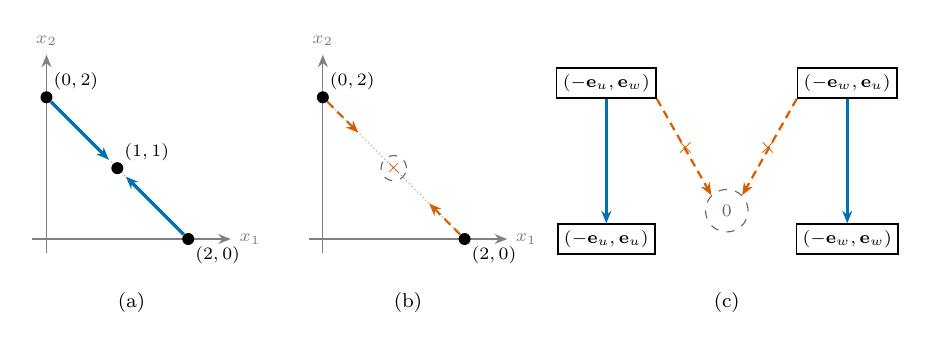
\begin{tikzpicture}[scale=0.9,transform shape,
  pt/.style={circle,fill=black,inner sep=1.7pt},
  hol/.style={circle,draw,dashed,black!60,inner sep=1.7pt},
  ax/.style={->,black!50},
  ex/.style={->,very thick,cA},
  bad/.style={->,thick,densely dashed,cB},
  st/.style={rectangle,draw,semithick,fill=white,inner sep=2.5pt,font=\scriptsize},
  lb/.style={font=\scriptsize}]
  \draw[ax] (-0.2,0) -- (2.6,0) node[right,lb] {$x_1$};
  \draw[ax] (0,-0.2) -- (0,2.6) node[above,lb] {$x_2$};
  \draw[black!35,densely dotted] (2,0) -- (0,2);
  \node[pt] (P) at (2,0) {};
  \node[pt] (Q) at (1,1) {};
  \node[pt] (R) at (0,2) {};
  \node[lb,below right=-1pt] at (P) {$(2,0)$};
  \node[lb,above right=-1pt] at (Q) {$(1,1)$};
  \node[lb,above right=-1pt] at (R) {$(0,2)$};
  \draw[ex] (P) -- (1.12,0.88);
  \draw[ex] (R) -- (0.88,1.12);
  \node[font=\footnotesize] at (1.2,-0.9) {(a)};
  \begin{scope}[xshift=3.9cm]
    \draw[ax] (-0.2,0) -- (2.6,0) node[right,lb] {$x_1$};
    \draw[ax] (0,-0.2) -- (0,2.6) node[above,lb] {$x_2$};
    \draw[black!35,densely dotted] (2,0) -- (0,2);
    \node[pt] (P2) at (2,0) {};
    \node[hol,minimum size=3.6mm] (Q2) at (1,1) {};
    \node[pt] (R2) at (0,2) {};
    \node[lb,below right=-1pt] at (P2) {$(2,0)$};
    \node[lb,above right=-1pt] at (R2) {$(0,2)$};
    \draw[bad] (P2) -- (1.5,0.5);
    \draw[bad] (R2) -- (0.5,1.5);
    \node[cB,font=\scriptsize] at (Q2) {$\times$};
    \node[font=\footnotesize] at (1.2,-0.9) {(b)};
  \end{scope}
  \begin{scope}[xshift=7.9cm]
    \node[st] (A) at (0,2.2) {$(-\e_u,\e_w)$};
    \node[st] (B) at (3.4,2.2) {$(-\e_w,\e_u)$};
    \node[st] (C) at (0,0) {$(-\e_u,\e_u)$};
    \node[st] (D) at (3.4,0) {$(-\e_w,\e_w)$};
    \node[hol,minimum size=6mm,font=\scriptsize] (O) at (1.7,0.4) {$0$};
    \draw[ex] (A) -- (C);
    \draw[ex] (B) -- (D);
    \draw[bad] (A.south east) -- (O.north west);
    \draw[bad] (B.south west) -- (O.north east);
    \node[cB,font=\small] at (1.12,1.28) {$\times$};
    \node[cB,font=\small] at (2.28,1.28) {$\times$};
    \node[font=\footnotesize] at (1.7,-0.9) {(c)};
  \end{scope}
\end{tikzpicture}
\caption{Trao đổi trong các tập M-lồi và việc loại bỏ trạng thái chết. (a) Tập $\{(2,0),(1,1),(0,2)\}$ là M-lồi; các điểm cực biên trao đổi hướng tới $(1,1)$. (b) Sau khi xóa $(1,1)$, không còn phép trao đổi nào. (c) Với digon trong Ví dụ~\ref{ex:digon}, phép trao đổi có thể kết thúc ở trạng thái chết $0$ (nét đứt) được thay bằng phép trao đổi từ $(-\e_u,\e_w)$ và $(-\e_w,\e_u)$ sang các trạng thái khác không $(-\e_u,\e_u)$ và $(-\e_w,\e_w)$.}
\label{fig:mconvex}
\end{figure}

Với $X\subseteq K$, gọi $\delta_K(X)$ là tập các cạnh của $K$ có đúng một đầu trong $X$. Trường hợp duy nhất có thể thất bại sau khi bỏ $0$ là một phép trao đổi được bảo đảm trong $\Gamma_K$ làm một trong hai trạng thái bằng không.

\begin{lemma}\label{lem:gamma}
\begin{enumerate}
\item[(a)] $\Gamma_K$ là M-lồi.
\item[(b)] Nếu $K$ là một thành phần chẵn (liên thông), thì $\Gamma'_K=\Gamma_K\setminus\{0\}$ là M-lồi.
\end{enumerate}
\end{lemma}

\begin{proof}
(a) Khẳng định này là cổ điển~\cite{hakimi1965,frank1980,frank2011}, chúng tôi chỉ quy nó về Bổ đề~\ref{lem:boundary}. Cố định một định hướng tham chiếu $R$ của $K$ với $d_R=\out-\inn$. Đảo cung $x\to y$ chuyển một cặp từ $y$ sang $x$, nên mọi định hướng cho $\beta-\alpha=\sigma+\partial\varphi$, trong đó $\sigma(v)=(p^{\inn}_v-p^{\out}_v-d_R(v))/2\in\Z$ và $\varphi\in\{0,1\}$ là hàm chỉ thị của các cung bị đảo của đồ thị có hướng $R^-$ thu được bằng cách đảo mọi cung của $R$. Xây dựng một mạng trên $K$ với các cung của $R^-$ có sức chứa $1$, cung cấp cố định $\sigma(v)$ tại mọi $v$, và với mỗi $v$ các đầu cuối $v_{\inn}$ và $v_{\out}$ cùng các cung không giới hạn $v_{\inn}\to v\to v_{\out}$. Các vector dòng vào ròng tại đầu cuối của nó chính xác là các điểm $(-\alpha,\beta)$ của $\Gamma_K$, là M-lồi theo Bổ đề~\ref{lem:boundary}.

(b) \emph{Ý tưởng.} Theo~(a) chỉ phép trao đổi tạo ra điểm $0$ mới gây vấn đề, chúng tôi chứng minh rằng khi đó tồn tại một chỉ số trao đổi khác, dùng tính đạt tới trong một định hướng của $g$ và một định hướng Euler liên thông mạnh. Mọi tính chẵn lẻ trong một thành phần chẵn đều bằng $0$, nên \eqref{eq:balance} trở thành $\inn_t-\out_t=2g$ với $g=\beta-\alpha$. Ta dùng hai hệ quả. Thứ nhất, cho $O$ thực hiện $g$ và $\emptyset\ne X\subsetneq K$. Vì $2g(v)=\inn_t(v)-\out_t(v)$, cộng trên $X$ sẽ triệt tiêu các cạnh nội bộ và cho $2g(X)=|\{\text{cut edges entering }X\}|-|\{\text{cut edges leaving }X\}|$. Do đó, nếu mọi cạnh của $\delta_K(X)$ đi vào $X$ thì $g(X)=|\delta_K(X)|/2>0$, còn nếu mọi cạnh như vậy đi ra thì $g(X)=-|\delta_K(X)|/2<0$, tính nghiêm ngặt theo tính liên thông của $K$. Thứ hai, mọi bậc trong $K$ đều chẵn, nên $K$ có chu trình Euler~\cite{hierholzer1873}. Định hướng thu được thực hiện $0$ và liên thông mạnh, nên $\e_v-\e_w$ khả thực hiện với mọi $v,w\in K$ theo Bổ đề~\ref{lem:reversal}.

Cho $x,y\in\Gamma'_K$ và $i$ là một tọa độ với $x_i>y_i$. Theo (a) có $j$ với $x_j<y_j$ sao cho $x'=x-\e_i+\e_j\in\Gamma_K$ và $y'=y+\e_i-\e_j\in\Gamma_K$. Nếu cả hai khác không thì xong. Chúng không thể đồng thời bằng không, vì khi đó $x=\e_i-\e_j=-y$, trong khi các tọa độ vào không dương và các tọa độ ra không âm, nên $i$ sẽ vừa là tọa độ ra ($x_i=1$) vừa là tọa độ vào ($y_i=-1$). Các điểm của $\Gamma_K$ thỏa $\alpha(K)=\beta(K)$, nên mọi điểm của $\Gamma'_K$ có $\alpha\ne0$ và $\beta\ne0$.

\emph{Trường hợp $x'=0$.} Khi đó $x=(-\e_u,\e_w)$, $i=w_{\out}$ và $j=u_{\inn}$. Viết $y=(-\alpha,\beta)$, đặt $g=\beta-\alpha$ và cho $O$ thực hiện $g$. Vì $y_i<1$, ta có $\beta_w=0$. Gọi $M$ là tập các đỉnh đi tới được từ $w$ trong $O$. Nếu $M\ne K$ thì mọi cạnh của $\delta_K(M)$ đi vào $M$, nên $\beta(M)\ge g(M)>0$. Nếu $M=K$ thì $\beta(K)\ge1$. Vậy có $z\in M\setminus\{w\}$ với $\beta_z\ge1$, vì $\beta_w=0$ và tổng dương $\beta(M)$ phải xuất hiện ở một đỉnh khác, đồng thời $g+\e_w-\e_z$ khả thực hiện theo Bổ đề~\ref{lem:reversal}. Lấy thay $j=z_{\out}$, thỏa $x_j=0<y_j$. Khi đó $x-\e_i+\e_j=(-\e_u,\e_z)\in\Gamma'_K$ theo hệ quả thứ hai, và $y+\e_i-\e_j\in\Gamma'_K$ vì hiệu của nó là $g+\e_w-\e_z$ và $\alpha\ne0$.

\emph{Trường hợp $y'=0$.} Khi đó $y=(-\e_u,\e_w)$, $i=u_{\inn}$ và $j=w_{\out}$. Viết $x=(-\alpha,\beta)$, đặt $g=\beta-\alpha$ và cho $O$ thực hiện $g$. Vì $x_i>-1$, ta có $\alpha_u=0$. Gọi $\Lambda$ là tập các đỉnh từ đó đi tới được $u$ trong $O$. Nếu $\Lambda\ne K$ thì mọi cạnh của $\delta_K(\Lambda)$ đi ra khỏi $\Lambda$, nên $\alpha(\Lambda)\ge-g(\Lambda)>0$. Nếu $\Lambda=K$ thì $\alpha(K)\ge1$. Vậy có $v\in\Lambda\setminus\{u\}$ với $\alpha_v\ge1$, vì $\alpha_u=0$ và tổng dương $\alpha(\Lambda)$ phải xuất hiện ở một đỉnh khác, đồng thời $g+\e_v-\e_u$ khả thực hiện theo Bổ đề~\ref{lem:reversal}. Lấy thay $j=v_{\inn}$, thỏa $x_j=-\alpha_v<0=y_j$. Khi đó $x-\e_i+\e_j$ chuyển một cặp vào từ $v$ sang $u$, hiệu của nó là $g+\e_v-\e_u$, và nó thuộc $\Gamma'_K$ (nó khác không vì tọa độ tại $u_{\inn}$ bằng $-1$). Cuối cùng $y+\e_i-\e_j=(-\e_v,\e_w)\in\Gamma'_K$ theo hệ quả thứ hai.
\end{proof}

\begin{remark}\label{rem:connected}
Tính liên thông là cần thiết trong Bổ đề~\ref{lem:gamma}(b): với hai tam giác rời nhau được coi là một thành phần duy nhất, tập tương ứng không là M-lồi. Nếu $g=\beta-\alpha$ được cố định trước rồi điểm $0$ bị bỏ đi, tiên đề trao đổi đã thất bại ngay với hai đỉnh nối bằng hai cạnh song song, nên bổ đề được phát biểu cho $\Gamma'_K$ với $g$ tự do.
\end{remark}

\subsection{Mạng cổng}\label{sec:ports}

Mỗi đỉnh $v$ trở thành một \emph{dòng thời gian} gồm các cổng. Gọi $K_1,\dots,K_{q_v}$ là các thành phần chứa các lần xuất hiện của $v$. Các cổng của $v$ là $S_v$ (bắt đầu), $\IN(K_j,v)$ và $\OUT(K_j,v)$ với $j=1,\dots,q_v$, và $Z_v$ (kết thúc). \emph{Các cung chờ} nối chúng theo thứ tự thời gian, cụ thể là $S_v\to\IN(K_1,v)$, $\OUT(K_j,v)\to\IN(K_{j+1},v)$ và $\OUT(K_{q_v},v)\to Z_v$. Một đỉnh không có cạnh chỉ có cung $S_v\to Z_v$. Một luồng $\xi\ge0$ trên một cung chờ là số cặp đang chờ tại $v$ giữa hai lần xuất hiện (Hình~\ref{fig:ports}). Với một cổng $P$, gọi $\partial\xi(P)$ là luồng ra khỏi $P$ trừ luồng vào $P$, có dấu ngược với luồng vào ròng $\partial\varphi$ trong chứng minh Bổ đề~\ref{lem:gamma}(a). Tại các cổng của một thành phần, $\partial\xi=(-\alpha,\beta)$.

Gọi $p_{\mathrm{end}}(v)$ là tính chẵn lẻ của $a_v+G_v$. Tập ràng buộc $\cB$ là tổng trực tiếp của các tập sau.
\begin{itemize}
\item Tại $S_v$, điểm duy nhất $\floor{a_v/2}$.
\item Tại các cổng của mỗi thành phần $K$, tập $\Gamma'_K$ nếu $K$ chẵn và $\Gamma_K$ trong trường hợp ngược lại.
\item Tại các cổng $Z_v$, với \FIX{}, điểm duy nhất $-(z_v-p_{\mathrm{end}}(v))/2$ tại mọi $v$, sau khi kiểm tra $z_v\equiv a_v+G_v \pmod 2$ và $z_v\ge p_{\mathrm{end}}(v)$. Với \FREE{}, đơn hình $\{-\gamma:\gamma\in\N^V,\ \gamma(V)=(k-\sum_vp_{\mathrm{end}}(v))/2\}$, chỉ cố định tổng số cặp cuối cùng.
\end{itemize}
Các điểm đơn và đơn hình cuối của \FREE{}, tức các điểm nguyên của đa diện cơ sở đều $\{-\gamma:\gamma\ge0,\ \gamma(V)=c\}$, là M-lồi~\cite{murota2003}. Theo Bổ đề~\ref{lem:boundary} và~\ref{lem:gamma}, $\cB$, tổng trực tiếp của chúng, là M-lồi. Nó khác rỗng sau các kiểm tra ở dòng 1 của Thuật toán~\ref{alg:pf}: các định hướng tùy ý cho trạng thái trong mỗi $\Gamma_K$, và nếu một thành phần chẵn nếu không sẽ có trạng thái không, thì thêm một cặp chờ tại cùng một đỉnh ở cả hai phía sẽ cho trạng thái khác không trong $\Gamma'_K$. Tập đầu và tập cuối khác rỗng nhờ các kiểm tra tính chẵn lẻ và tổng số lượng. Vì $\sum_v(a_v+G_v)=k+2m$, số $k-\sum_vp_{\mathrm{end}}(v)$ luôn chẵn.

Ví dụ chạy: xét Hình~\ref{fig:aaai}(a) với một walk xuất phát tại mỗi đỉnh $x$ và $y$ và đầu cuối tự do. Hình~\ref{fig:overview} mô tả ba giai đoạn của ví dụ này. Hình~\ref{fig:ports} biểu diễn mạng cổng cho instance \FREE{} này và một đường tăng (các mũi tên đậm màu xanh đánh số $1$--$5$) sửa tam giác chết của nó, $+1$ và $-1$ đánh dấu các độ lệch khác không, và $\eta$ thực hiện một phép trao đổi giữa các cổng kết thúc.

\begin{figure}[!tb]
\centering
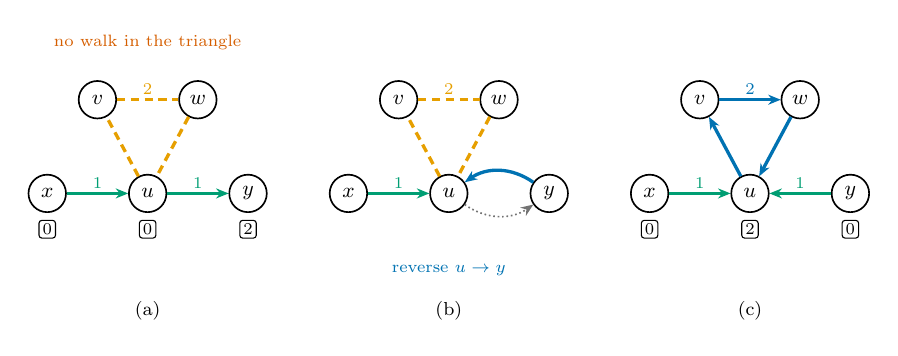
\begin{tikzpicture}[scale=0.85,transform shape,
  el/.style={font=\scriptsize,inner sep=1.5pt},
  old/.style={->,semithick,densely dotted,black!55},
  hl/.style={->,very thick,cA}]
  \foreach \o/\p in {0/a,4.5/b,9.0/c} {
    \node[vtx] (x\p) at (\o,0)     {$x$};
    \node[vtx] (u\p) at (\o+1.5,0) {$u$};
    \node[vtx] (y\p) at (\o+3,0)   {$y$};
    \node[vtx] (v\p) at (\o+0.75,1.4) {$v$};
    \node[vtx] (w\p) at (\o+2.25,1.4) {$w$};
  }
  \draw[t1,->] (xa) -- node[el,above] {1} (ua);
  \draw[t1,->] (ua) -- node[el,above] {1} (ya);
  \draw[t2] (ua) -- (va);
  \draw[t2] (va) -- node[el,above] {2} (wa);
  \draw[t2] (wa) -- (ua);
  \node[cnt,below=3pt of xa] {0};
  \node[cnt,below=3pt of ua] {0};
  \node[cnt,below=3pt of ya] {2};
  \node[note,text=cB] at (1.5,2.25) {no walk in the triangle};
  \draw[t1,->] (xb) -- node[el,above] {1} (ub);
  \draw[old] (ub) to[bend right=35] (yb);
  \draw[hl] (yb) to[bend right=35] (ub);
  \draw[t2] (ub) -- (vb);
  \draw[t2] (vb) -- node[el,above] {2} (wb);
  \draw[t2] (wb) -- (ub);
  \node[note,text=cA] at (6.0,-1.15) {reverse $u\to y$};
  \draw[t1,->] (xc) -- node[el,above] {1} (uc);
  \draw[t1,->] (yc) -- node[el,above] {1} (uc);
  \draw[walkA] (uc) -- (vc);
  \draw[walkA] (vc) -- node[el,above] {2} (wc);
  \draw[walkA] (wc) -- (uc);
  \node[cnt,below=3pt of xc] {0};
  \node[cnt,below=3pt of uc] {2};
  \node[cnt,below=3pt of yc] {0};
  \node[font=\footnotesize] at (1.5,-1.75) {(a)};
  \node[font=\footnotesize] at (6.0,-1.75) {(b)};
  \node[font=\footnotesize] at (10.5,-1.75) {(c)};
\end{tikzpicture}
\caption{Tổng quan thuật toán trên ví dụ chạy. Các hộp cho biết số walk tại mỗi đỉnh sau thời điểm 1: $x:0$, $u:0$, $y:2$ ở (a) và $x:0$, $u:2$, $y:0$ ở (c). (a) Sau luồng cực đại, các cạnh thời điểm 1 khiến $u$ không còn walk, nên tam giác thời điểm 2 bị chết. (b) Một đường tăng đảo hướng cạnh $u\to y$. (c) Sau khi tăng luồng, $u$ có hai walk: $x\to u\to v\to w\to u$ và $y\to u$.}
\label{fig:overview}
\end{figure}

\begin{figure}[!htbp]
\centering
\begin{tikzpicture}[scale=0.8,transform shape,x=1.12cm,y=0.9cm,
  wait/.style={->,black!55,semithick},
  aug/.style={->,cA,line width=1.6pt},
  stp/.style={circle,fill=cA,text=white,font=\scriptsize\bfseries,inner sep=0.8pt,minimum size=3.4mm},
  hdr/.style={font=\scriptsize,text=black!70}]
  \def\cS{0} \def\cIa{1.7} \def\cOa{2.9} \def\cIb{4.9} \def\cOb{6.1} \def\cZ{7.9}
  \foreach \v/\Y in {x/2,y/1,u/0,v/-1,w/-2} {
    \node[font=\small] at (-0.55,\Y) {$\v$};
    \node[port] (S-\v) at (\cS,\Y) {};
    \node[port] (Z-\v) at (\cZ,\Y) {};
  }
  \foreach \v/\Y in {x/2,y/1,u/0} { \node[port] (I1-\v) at (\cIa,\Y) {}; \node[port] (O1-\v) at (\cOa,\Y) {}; }
  \foreach \v/\Y in {u/0,v/-1,w/-2} { \node[port] (I2-\v) at (\cIb,\Y) {}; \node[port] (O2-\v) at (\cOb,\Y) {}; }
  \begin{scope}[on background layer]
    \draw[cTa,semithick,rounded corners=2pt,fill=cTa!7] (\cIa-0.38,-0.42) rectangle (\cOa+0.38,2.42);
    \draw[cB,semithick,densely dashed,rounded corners=2pt,fill=cB!6] (\cIb-0.38,-2.42) rectangle (\cOb+0.38,0.42);
  \end{scope}
  \node[hdr] at (\cS,2.85) {$S_v$};
  \node[hdr] at (\cZ,2.85) {$Z_v$};
  \node[hdr] at (\cIa,2.85) {$\IN$};
  \node[hdr] at (\cOa,2.85) {$\OUT$};
  \node[hdr] at (\cIb,-2.85) {$\IN$};
  \node[hdr] at (\cOb,-2.85) {$\OUT$};
  \node[font=\scriptsize] at ({(\cIa+\cOa)/2},3.35) {thành phần tại thời điểm $1$: $\Gamma_K$};
  \node[font=\scriptsize] at ({(\cIb+\cOb)/2},-3.35) {thành phần tại thời điểm $2$: $\Gamma'_K$ (chẵn, chết)};
  \foreach \v in {x,y,u} \draw[wait] (S-\v) -- (I1-\v);
  \foreach \v in {v,w} \draw[wait] (S-\v) -- (I2-\v);
  \foreach \v in {x,y} \draw[wait] (O1-\v) -- (Z-\v);
  \draw[wait] (O1-u) -- (I2-u);
  \foreach \v in {u,v,w} \draw[wait] (O2-\v) -- (Z-\v);
  \node[circle,draw=black!55,fill=white,font=\scriptsize,inner sep=1pt] (eta) at (9.0,0.5) {$\eta$};
  \foreach \v in {x,y,u,v,w} \draw[black!40,thin,densely dashed] (Z-\v) -- (eta);
  \node[font=\scriptsize,above=1pt] at (7.0,1) {$\xi=1$};
  \node[font=\scriptsize,below=1pt] at (I2-u.south) {$+1$};
  \node[font=\scriptsize,below=1pt] at (O2-u.south) {$-1$};
  \draw[aug] ([yshift=-3pt]I2-u.west) -- node[stp,below=2pt] {1} ([yshift=-3pt]O1-u.east);
  \draw[aug] ([xshift=3pt]O1-u.north) -- node[stp,right=2pt] {2} ([xshift=3pt]O1-y.south);
  \draw[aug] ([yshift=-3pt]O1-y.east) -- node[stp,below=2pt,pos=0.86] {3} ([yshift=-3pt]Z-y.west);
  \draw[aug,-] (Z-y.east) -- (eta);
  \draw[aug] (eta) -- (Z-u.east);
  \node[stp] at ($(eta)+(0.45,0)$) {4};
  \draw[aug] ([yshift=-3pt]Z-u.west) -- node[stp,below=2pt] {5} ([yshift=-3pt]O2-u.east);
\end{tikzpicture}
\caption{Mạng cổng và đường tăng cho ví dụ \FREE{} đang xét.}
\label{fig:ports}
\end{figure}

\begin{theorem}\label{thm:reduction}
Một instance của \FREE{} hoặc \FIX{} khả thi khi và chỉ khi có một luồng cặp $\xi\ge0$ trên các cung chờ với $\partial\xi\in\cB$.
\end{theorem}

\begin{proof}
($\Rightarrow$) Lấy định hướng của các walk và đặt $\xi=q$ trên mọi cung chờ. Tại $S_v$ ta có $\partial\xi=\floor{a_v/2}$. Tại mỗi thành phần, $\partial\xi=(-\alpha,\beta)$ với $\beta\ge0$ theo (i), hiệu $\beta-\alpha$ được chính định hướng đó thực hiện, và $(-\alpha,\beta)\ne0$ trên các thành phần chẵn theo (ii). Tại $Z_v$, giá trị $-\partial\xi$ là số cặp cuối cùng tại $v$. Nó bằng $(z_v-p_{\mathrm{end}}(v))/2$ trong \FIX{}, và trong \FREE{} các giá trị này có tổng $(k-\sum_vp_{\mathrm{end}}(v))/2$ vì số walk được bảo toàn.

($\Leftarrow$) Với mỗi $K$ chọn một định hướng thực hiện $\beta-\alpha$. Theo~\eqref{eq:balance}, số walk tại $v$ giữa hai lần xuất hiện dưới định hướng kết hợp bằng $2\xi+p$ trên cung chờ tương ứng. Điều kiện (i) đúng vì $\beta\ge0$. Điều kiện (ii) đúng trên các thành phần không chẵn theo Bổ đề~\ref{lem:noneven}, và trên các thành phần chẵn vì $(-\alpha,\beta)\ne0$. Với \FIX{}, số walk cuối cùng tại $v$ là $z_v$. Định lý~\ref{thm:char} hoàn tất chứng minh.
\end{proof}

Tương đương, Định lý~\ref{thm:reduction} hỏi liệu tập M-lồi $\{\partial\xi:\xi\ge0\}$ các biên của luồng chờ không âm (M-lồi theo Bổ đề~\ref{lem:boundary}, sai khác dấu) có giao với tập M-lồi $\cB$ hay không, đây là một instance khả thi của giao M-lồi~\cite{murota2003,edmonds1977,franktardos1988}.

\subsection{Thuật toán đường tăng}\label{sec:auxgraph}

Thuật toán khởi tạo $\xi$ từ định hướng luồng chuỗi: trên mỗi cung chờ đặt số cặp (một nửa bộ đếm walk, là số nguyên theo tính chẵn lẻ cố định), các tọa độ IN và OUT của mỗi thành phần trong $x$ là $-\alpha$ và $\beta$ từ định hướng đó, $x(S_v)=\lfloor a_v/2\rfloor$, và tọa độ cuối bằng âm số cặp cuối cùng. Với mỗi thành phần chẵn ban đầu chết, dòng 3 thay trạng thái không của nó bằng một cặp vào và một cặp ra tại một đỉnh được chọn. Thuật toán duy trì một luồng $\xi\ge0$ và một điểm $x\in\cB$. \emph{Độ lệch} của chúng là $d=\partial\xi-x$. Lời giải thu được khi $d=0$. \emph{Đồ thị phụ} có các cổng làm nút và ba loại cung, mỗi cung chuyển một đơn vị độ lệch từ đuôi sang đầu.
\begin{enumerate}
\item[(1)] Đảo ngược của mọi cung chờ. Dùng nó làm tăng $\xi$ trên cung đó thêm một.
\item[(2)] Mọi cung chờ có $\xi>0$. Dùng nó làm giảm $\xi$ đi một.
\item[(3)] Một cung trao đổi $i\to j$ bất cứ khi nào $x+\e_i-\e_j\in\cB$. Dùng nó thay $x$ bằng $x+\e_i-\e_j$.
\end{enumerate}
Giả sử $i$ là một cổng của $v$ và $j$ là một cổng của $w$ trong cùng thành phần $K$. Cung trao đổi $i\to j$ tồn tại khi và chỉ khi $\alpha_v\ge1$ khi $i$ là cổng vào, $\beta_w\ge1$ khi $j$ là cổng ra, $v=w$ hoặc định hướng hiện tại của $K$ có một đường có hướng từ $v$ đến $w$ (Bổ đề~\ref{lem:reversal}), và nếu $K$ chẵn thì điểm mới khác không. Không cần điều kiện khả dụng khi $i$ là cổng ra hoặc $j$ là cổng vào, vì các thay đổi đó làm tăng số cặp tương ứng. Trong đơn hình của \FREE{}, $x+\e_i-\e_j\in\cB$ bất cứ khi nào $\gamma_i\ge1$. Thay vì $\Theta(n^2)$ cung này, đồ thị phụ chứa một nút $\eta$ với các cung $Z_i\to\eta$ với mọi $i$ có $\gamma_i\ge1$ và $\eta\to Z_j$ với mọi $j$, và một đường qua $\eta$ thực hiện một phép trao đổi đơn hình. Có thể dùng đường ngắn nhất bất kỳ và chọn đỉnh bất kỳ ở dòng 3. Hình~\ref{fig:aux} minh họa ba loại cung và chứng nhận dùng trong Định lý~\ref{thm:correct}.

\begin{figure}[!tb]
\centering
\begin{tikzpicture}[x=1cm,y=1cm,font=\scriptsize,
  box/.style={black!45,rounded corners=2pt},
  wait/.style={->,black!55,semithick},
  ka/.style={->,cA,thick},
  kb/.style={->,cB,thick,densely dashed},
  kc/.style={->,cTa,thick}]
  \draw[box] (-0.4,-0.45) rectangle (1.9,1.55);
  \node[anchor=south] at (0.75,1.55) {thành phần $K$};
  \draw[box] (3.4,-0.45) rectangle (4.4,1.55);
  \node[anchor=south] at (3.9,1.55) {$K'$};
  \node[port,label=left:$i$] (i) at (0.1,1.0) {};
  \node[port,label=right:$j$] (j) at (1.4,1.0) {};
  \node[port,label=left:$P$] (P) at (1.4,0) {};
  \node[port,label=right:$Q$] (Q) at (3.9,0) {};
  \draw[wait] (P) -- node[pos=0.72,above=-1pt,black] {$\xi$} (Q);
  \draw[ka] (Q) to[bend right=40] node[above=-1pt] {(1)\ $\xi{+}1$} (P);
  \draw[kb] (P) to[bend right=40] node[below=-1pt] {(2)\ $\xi{-}1$, nếu $\xi>0$} (Q);
  \draw[kc] (i) -- node[above=-1pt] {(3)} (j);
  \node[font=\small] at (-0.75,1.75) {(a)};
  \begin{scope}[xshift=6.1cm]
    \draw[cA,fill=cA!7,rounded corners=6pt] (-0.3,-0.45) rectangle (1.9,1.55);
    \node[cA] at (-0.05,1.3) {$R$};
    \node[port,label=below:{$d>0$}] (p) at (0.35,0.55) {};
    \node[port] (r) at (1.45,1.0) {};
    \node[port] (s) at (1.45,0.0) {};
    \node[port,label=right:{$d<0$}] (n) at (3.6,1.0) {};
    \node[port] (o) at (3.6,0.0) {};
    \draw[kc] (p) -- (r);
    \draw[kc] (n) to[bend right=12] (r);
    \draw[wait] (s) -- node[below=-1pt,black] {$\xi=0$} (o);
    \draw[->,black!40,thick] (r) to[bend left=50] node[black,font=\small] {$\times$} (n);
    \node[font=\small] at (-0.65,1.75) {(b)};
  \end{scope}
\end{tikzpicture}
\caption{Đồ thị phụ. (a) Ba loại cung tại một cung chờ $P\to Q$ có luồng $\xi$ và tại hai cổng $i,j$ của cùng một thành phần, trong đó loại~(3) đòi hỏi $x+\e_i-\e_j\in\cB$; mỗi cung chuyển một đơn vị độ lệch từ đuôi sang đầu của nó. (b) Chứng nhận của Định lý~\ref{thm:correct}: tập $R$ các cổng khả đạt từ $\{d>0\}$ không chứa cổng nào có $d<0$, và không có cung nào rời $R$. Khi đó $x(R)=-d(R)<0$, trong khi Bổ đề~\ref{lem:localmax} cho $x(R)\ge x'(R)\ge0$ với mọi lời giải $(\xi',x')$.}
\label{fig:aux}
\end{figure}

\begin{algorithm}[t]
\caption{Thuật toán đường tăng cho \FIX{} và \FREE{}}\label{alg:pf}
\begin{algorithmic}[1]
\State Kiểm tra các điều kiện đếm ($\sum a=\sum z$ và $h_v\in\N$ với \FIX{}, $k\ge\sum_vp_{\mathrm{end}}(v)$ với \FREE{}). \textbf{nếu} một kiểm tra thất bại \textbf{thì trả về} \NO{}.
\State Giải một luồng cực đại trong mạng chuỗi. \textbf{nếu} giá trị của nó nhỏ hơn $m$ \textbf{thì trả về} \NO{} cùng với lát cắt nhỏ nhất.
\State Lấy định hướng của luồng cực đại và $\xi$, $x$ cảm sinh. Với mỗi thành phần chẵn chết $K$, chọn $v\in K$, đặt $x=(-\e_v,\e_v)$ tại $(\IN(K,v),\OUT(K,v))$, để có $d=+1$ tại $\IN(K,v)$ và $d=-1$ tại $\OUT(K,v)$.
\While{tồn tại cổng có $d>0$}
  \State Tìm một đường \emph{ngắn nhất} từ $\{d>0\}$ đến $\{d<0\}$ trong đồ thị phụ bằng tìm kiếm theo chiều rộng.
  \If{không tồn tại đường như vậy}
    \State \Return \NO{} cùng với tập $R$ các cổng khả đạt từ $\{d>0\}$.
  \EndIf
  \State Áp dụng đồng thời tất cả các cung của đường vào $\xi$ và $x$, rồi định hướng lại các thành phần có điểm thay đổi (xem bên dưới).
\EndWhile
\State \Return \YES{} và xây dựng các walk như trong chứng minh Định lý~\ref{thm:char}.
\end{algorithmic}
\end{algorithm}

Trong phép định hướng lại đạt cận định lý, ta lặp lại việc đảo một đường có hướng từ một đỉnh có bậc vào đích lớn hơn bậc vào hiện tại đến một đỉnh có bậc vào hiện tại lớn hơn đích, điều này làm giảm khoảng cách $L_1$ tới đích đi hai, $O(|K|)$ đường, mỗi đường tốn thời gian $O(m_K)$, là đủ cho một thành phần $K$.

\subsection{Tính đúng và các chứng nhận vô nghiệm}

\begin{lemma}\label{lem:invariant}
Sau mỗi lần tăng, $\xi\ge0$ và $x\in\cB$.
\end{lemma}

\begin{proof}
Mọi cung của đường được đánh giá tại trạng thái trước khi tăng và được áp dụng cùng lúc. Một đường ngắn nhất là đơn, nên mỗi cung chờ được dùng nhiều nhất một lần và các cung loại~(2) chỉ được dùng khi $\xi>0$. Do đó $\xi\ge0$. Một đường đơn ghé $\eta$ nhiều nhất một lần, nên đơn hình của \FREE{} trải qua nhiều nhất một phép trao đổi, và phép này hợp lệ theo định nghĩa các cung. Xét một hạng tử khác $\Gamma$ của $\cB$ và các phép trao đổi $(i_1,j_1),\dots,(i_r,j_r)$ của nó theo thứ tự trên đường. Các nút của một đường ngắn nhất có khoảng cách tìm kiếm theo chiều rộng từ tập $\{d>0\}$ đôi một khác nhau và tăng dần, nên các $i_l$ đôi một khác nhau và các $j_l$ đôi một khác nhau. Nếu tồn tại $l<l'$ với một cung $i_l\to j_{l'}$, thì $\mathrm{dist}(j_{l'})\le\mathrm{dist}(i_l)+1<\mathrm{dist}(i_{l'})+1=\mathrm{dist}(j_{l'})$, mâu thuẫn. Vậy giả thiết của Bổ đề~\ref{lem:exchange} được thỏa. Lập luận chỉ dùng thứ tự của các khoảng cách, nên không bị ảnh hưởng khi đường đi vào và rời cùng một thành phần nhiều lần, và bổ đề được áp dụng cho chính $\Gamma'_K$, là M-lồi theo Bổ đề~\ref{lem:gamma}. Theo Bổ đề~\ref{lem:exchange}, điểm mới vẫn nằm trong tập.
\end{proof}

\begin{theorem}\label{thm:correct}
Thuật toán~\ref{alg:pf} trả lời đúng. Khi nó trả lời \YES{}, các walk trả về tạo thành một lời giải. Khi nó trả lời \NO{} trong vòng lặp, tập $R$ các cổng khả đạt từ $\{d>0\}$ chứng nhận vô nghiệm.
\end{theorem}

\begin{proof}
\NO{} ở dòng~2 là đúng vì (i) là điều kiện cần. Tổng của $d$ trên mọi cổng bằng $0$ sau dòng~3 (các phần tử khác không duy nhất là $+1$ và $-1$ của các thành phần chết được sửa) và vẫn bằng $0$, vì mỗi cung của đồ thị phụ chuyển một đơn vị giữa hai cổng, nên nếu vòng lặp kết thúc thì $d=0$, $\partial\xi=x\in\cB$ với $\xi\ge0$ theo Bổ đề~\ref{lem:invariant}, và các walk được xây dựng qua Định lý~\ref{thm:reduction}. Giả sử thuật toán dừng với tập $R$. Nó chứa mọi cổng có $d>0$ và không chứa cổng nào có $d<0$, nên $d(R)>0$. Không có cung nào của đồ thị phụ rời khỏi $R$. Theo loại~(1), không có cung chờ nào đi vào $R$, và theo loại~(2), mọi cung chờ rời khỏi $R$ đều có $\xi=0$. Do đó $\partial\xi(R)=0$ và $x(R)=-d(R)<0$. Vì $x\in\cB$ và $\xi\ge0$ trong suốt quá trình (Bổ đề~\ref{lem:invariant}), giả sử có một lời giải $(\xi',x')$ với $\xi'\ge0$ và $x'=\partial\xi'\in\cB$. Vì không có cung chờ nào đi vào $R$, $x'(R)$ là tổng của $\xi'$ trên các cung chờ rời khỏi $R$, nên $x'(R)\ge0$. Không có cung trao đổi nào rời khỏi $R$. Với đơn hình, điều này đúng vì một cổng $Z_i\in R$ với $\gamma_i\ge1$ đưa $\eta$ và mọi $Z_j$ vào $R$. Bổ đề~\ref{lem:localmax}, áp dụng cho từng hạng tử của tổng trực tiếp, cho $x(R)\ge x'(R)\ge0$, mâu thuẫn.
\end{proof}

Với mọi câu trả lời \YES{}, cài đặt xây dựng các walk và kiểm tra chúng theo định nghĩa bài toán. Câu trả lời \NO{} ở dòng~2 có một chứng nhận lát cắt của mạng chuỗi, có thể kiểm tra chỉ từ dữ liệu instance. Với một \NO{} trong vòng lặp, bộ kiểm tra xác minh $\xi,x$, tính $d=\partial\xi-x$, kiểm tra $d(R)>0$, và xác nhận không có cung chờ hay cung trao đổi hợp lệ nào rời khỏi $R$. Chứng nhận này không phụ thuộc Bổ đề~\ref{lem:exchange}, vì $x\in\cB$ được kiểm tra lúc chạy, nhưng nó phụ thuộc Bổ đề~\ref{lem:gamma} và~\ref{lem:localmax}, nên việc xác minh nó là phụ thuộc lý thuyết.

\subsection{Độ phức tạp}

\begin{theorem}\label{thm:time}
Gọi $D$ là số thành phần chẵn chết sau luồng cực đại và $s$ là số đỉnh lớn nhất của một thành phần snapshot. Thuật toán~\ref{alg:pf} thực hiện nhiều nhất $D$ lần tăng và dùng
\[
  O\bigl(n+m\log(m+1)+m^2+D\,(n+s\,m)\bigr)\subseteq O(n+n\,m^2)
\]
phép toán số học, vì $D\le m/2$ và $s\le n$.
\end{theorem}

\begin{proof}
Mỗi lần tăng làm tổng các độ lệch dương giảm đúng một, và tổng này bằng $D$ sau dòng~3. Các thành phần chẵn chết phân biệt không có cạnh chung, và mỗi thành phần có ít nhất hai cạnh, nên $D\le m/2$. Các dòng 1 đến 3 tốn $O(n+m^2)$ phép toán số học, bị chi phối bởi luồng cực đại ban đầu: mạng chuỗi có $O(m)$ nút và cung và giá trị luồng không vượt quá $m$, nên nhiều nhất $m$ đường tăng, mỗi đường tốn $O(m)$ thời gian, là đủ. Một lần tăng tốn $O(n+sm)$. Số cổng là $O(n+m)$, nên tìm kiếm theo chiều rộng trên đồ thị phụ tốn $O(n+m)$ thời gian, chưa kể các phép thử trao đổi. Với một thành phần $K$ có $m_K$ cạnh, tìm kiếm theo chiều sâu từ mỗi đỉnh của $K$ tốn $O(\abs{K}\,m_K)$ thời gian, và $O(\abs{K}^2)$ cặp trao đổi ứng viên cũng có cùng chi phí, vì $\abs{K}\le m_K+1$. Định hướng lại một thành phần $K$ bị thay đổi cần $O(\abs{K})$ phép đảo đường, mỗi phép tốn $O(m_K)$ thời gian, vì các phép trao đổi bên trong $K$ dùng các cổng phân biệt và $K$ có $2\abs{K}$ cổng: đảo một đường từ một đỉnh thặng dư đến một đỉnh thiếu hụt làm khoảng cách $L_1$ đến biên đích giảm hai (Bổ đề~\ref{lem:reversal}). Lấy tổng trên các thành phần, $\sum_K\abs{K}\,m_K\le sm$.
\end{proof}

Cận không phụ thuộc vào độ lớn của $a$ và $z$: mọi số được xử lý đều là số nguyên có giá trị tuyệt đối $O(k+m)$, nên cận này cũng là đa thức theo kích thước đầu vào tính bằng bit. Khi $D=0$ thuật toán chỉ là một luồng cực đại. Giá trị $D$ phụ thuộc vào luồng cực đại ban đầu, vì định hướng của bất kỳ lời giải nào cũng chính là một luồng cực đại với $D=0$.

\section{Walk chặt là NP-đầy đủ}\label{sec:strict}

Một walk \emph{chặt} có nhãn thời gian tăng nghiêm ngặt và dùng nhiều nhất một cạnh của mỗi snapshot. Gọi \SFIX{} và \SFREE{} là các biến thể chặt của \FIX{} và \FREE{}. Trường hợp đỉnh kết thúc cho trước được Deligkas và cộng sự để mở~\cite[p.~26504]{deligkas2025}, ngoài các trường hợp đặc biệt ở Mục~\ref{sec:related}.

\subsection{Các định hướng khả thi}

Một walk chặt đến một đỉnh tại thời điểm $t$ không thể rời đỉnh đó tại thời điểm $t$.

\begin{lemma}\label{lem:strict}
Một định hướng là khả thi bởi các walk chặt xuất phát theo $a$ khi và chỉ khi $\out_t(v)\le c_t(v)$ với mọi đỉnh $v$ và mọi thời điểm $t$. Với \SFIX{}, số walk cuối cùng tại $v$ còn phải bằng $z_v$ với mọi $v$.
\end{lemma}

\begin{proof}
\emph{Điều kiện cần.} Một walk chặt dùng nhiều nhất một cạnh tại thời điểm $t$. Vì vậy $\out_t(v)$ cung rời $v$ tại thời điểm $t$ được đi qua bởi các walk đôi một khác nhau, và mỗi walk trong số đó nằm tại $v$ ngay trước $t$. \emph{Điều kiện đủ.} Xử lý các thời điểm theo thứ tự tăng dần. Tại thời điểm $t$, gán cho các cung rời $v$ các walk đôi một khác nhau đang nằm tại $v$, điều này tồn tại vì $\out_t(v)\le c_t(v)$. Mỗi walk trong số này đi qua cung của nó, và mọi walk khác chờ. Số walk tại mọi đỉnh sau $t$ bằng $c_{t^+}$, nên quy nạp tiếp tục.
\end{proof}

So với Định lý~\ref{thm:char}, điều kiện (i) được thay bằng điều kiện mạnh hơn $\out_t(v)\le c_t(v)$, và điều kiện (ii) biến mất, vì mọi cạnh đều được đi qua bởi một walk đã ở đuôi của nó trước đó. Do đó một định hướng thỏa mãn điều kiện chặt không có thành phần chẵn chết. Trong ký hiệu của Mục~\ref{sec:char}, điều kiện mới là $2B_{v,j-1}+b_{v,j}\le a_v+G_{v,j-1}$, các trọng số khác nhau của các lần rời đi hiện tại và trước đó khiến không thể biểu diễn nó bằng một ràng buộc sức chứa của mạng chuỗi.

\subsection{Phép quy}

Chúng tôi quy từ bài toán thỏa mãn được với các mệnh đề gồm hai hoặc ba literal, trong đó mỗi biến xuất hiện nhiều nhất ba lần, là NP-đầy đủ theo Tovey~\cite{tovey1984}. Có thể giả sử các literal của một mệnh đề thuộc các biến khác nhau (loại các mệnh đề hằng đúng, gộp các literal lặp, lan truyền các mệnh đề đơn vị), và mỗi literal xuất hiện nhiều nhất hai lần: một literal xuất hiện ba lần là literal thuần (pure), vì biến của nó xuất hiện nhiều nhất ba lần nên literal đối lập không xuất hiện, do đó ta đặt nó bằng đúng và xóa các mệnh đề chứa nó, việc này không tạo ra lần xuất hiện mới nào và không tạo mệnh đề cỡ $1$. Gọi $\varphi$ là một công thức như vậy với các biến $x_1,\dots,x_{n_\varphi}$ và các mệnh đề $C_1,\dots,C_{m_\varphi}$. Gọi $s_j\in\{2,3\}$ là số literal của $C_j$ và $d(\ell)\le2$ là số mệnh đề chứa literal $\ell$. Vì $\sum_js_j=\sum_\ell d(\ell)\le4n_\varphi$ và $s_j\ge2$, ta có $m_\varphi\le2n_\varphi$. Đồ thị thời gian $G_\varphi$ có một đỉnh cho mỗi trong $2n_\varphi$ literal, một đỉnh cho mỗi mệnh đề, một \emph{trung tâm} $h$, và các đỉnh bậc một gọi là \emph{lá}. Các cạnh của nó như sau (Hình~\ref{fig:strict}).
\begin{itemize}
\item \emph{Thời điểm $1$.} Một \emph{lá xuất phát} được nối với mỗi đỉnh literal, $s_j-1$ lá xuất phát được nối với $C_j$, và $4n_\varphi$ lá xuất phát được nối với $h$.
\item \emph{Thời điểm $2$.} Cạnh $\{x_i,\lnot x_i\}$ với mỗi biến $x_i$.
\item \emph{Thời điểm $3$.} Cạnh $\{C_j,\ell\}$ với mỗi mệnh đề $C_j$ và mỗi literal $\ell$ của $C_j$.
\item \emph{Thời điểm $4$ và $5$.} Một cạnh $\{\ell,h\}$ tại thời điểm $4$ và một cạnh tại thời điểm $5$, với mỗi đỉnh literal $\ell$.
\item \emph{Thời điểm $6$.} $d(\ell)$ \emph{lá kết thúc} được nối với mỗi đỉnh literal $\ell$, một lá kết thúc được nối với mỗi $C_j$, và $6n_\varphi-2m_\varphi$ lá kết thúc được nối với $h$.
\end{itemize}
Ta đặt $a_v=1$ tại mọi lá xuất phát, $z_v=1$ tại mọi lá kết thúc, và $a_v=z_v=0$ trong các trường hợp khác. Có $6n_\varphi+\sum_js_j-m_\varphi$ lá xuất phát và cũng bấy nhiêu lá kết thúc. Đồ thị $G_\varphi$ không có cạnh song song trong một snapshot, và kích thước của nó tuyến tính theo kích thước của $\varphi$.

Trong Hình~\ref{fig:strict}, nhãn cạnh là thời gian và số bên cạnh một lá cho biết bội số của nó. Lá trắng là lá xuất phát và lá tô màu là lá kết thúc. Các liên thuộc mệnh đề khác và các lá kết thúc của $\lnot x_i$ được lược bỏ.

\begin{figure}[!htbp]
\centering
\begin{tikzpicture}[scale=0.8,transform shape,
  lit/.style={circle,draw,semithick,fill=white,minimum size=6.4mm,inner sep=0pt,font=\footnotesize},
  leaf/.style={circle,draw,semithick,fill=white,minimum size=1.8mm,inner sep=0pt},
  eleaf/.style={circle,draw,semithick,fill=black!55,minimum size=1.8mm,inner sep=0pt},
  ed/.style={semithick},
  lab/.style={fill=white,inner sep=0.8pt,font=\scriptsize}]
  \node[lit] (x)  at (0,1.1)  {$x_i$};
  \node[lit] (nx) at (0,-1.1) {$\lnot x_i$};
  \node[lit] (c)  at (3.4,1.1) {$C_j$};
  \node[lit] (h)  at (3.4,-1.1) {$h$};
  \draw[ed] (x) -- node[lab] {2} (nx);
  \draw[ed] (x) -- node[lab] {3} (c);
  \draw[ed] (x) to[bend left=10] node[lab,pos=0.42] {4} (h);
  \draw[ed] (x) to[bend right=10] node[lab,pos=0.62] {5} (h);
  \draw[ed] (nx) to[bend left=12] node[lab] {4} (h);
  \draw[ed] (nx) to[bend right=12] node[lab] {5} (h);
  \node[leaf] (sx) at (-1.3,1.1) {};
  \node[leaf] (snx) at (-1.3,-1.1) {};
  \draw[ed] (sx) -- node[lab] {1} (x);
  \draw[ed] (snx) -- node[lab] {1} (nx);
  \node[eleaf] (ex) at (-0.9,2.1) {};
  \draw[ed] (x) -- node[lab] {6} (ex);
  \node[note,anchor=east] at (-1.05,2.1) {$d(x_i)$};
  \node[leaf] (sc) at (3.4,2.3) {};
  \draw[ed] (sc) -- node[lab] {1} (c);
  \node[note,anchor=west] at (3.55,2.3) {$s_j-1$};
  \node[eleaf] (ec) at (4.7,1.1) {};
  \draw[ed] (c) -- node[lab] {6} (ec);
  \node[leaf] (sh) at (4.7,-0.6) {};
  \draw[ed] (sh) -- node[lab] {1} (h);
  \node[note,anchor=west] at (4.85,-0.6) {$4n_\varphi$};
  \node[eleaf] (eh) at (4.7,-1.6) {};
  \draw[ed] (h) -- node[lab] {6} (eh);
  \node[note,anchor=west] at (4.85,-1.6) {$6n_\varphi-2m_\varphi$};
  \node[leaf] at (6.9,1.6) {};
  \node[note,anchor=west] at (7.05,1.6) {lá xuất phát ($a=1$)};
  \node[eleaf] at (6.9,1.1) {};
  \node[note,anchor=west] at (7.05,1.1) {lá kết thúc ($z=1$)};
\end{tikzpicture}
\caption{Phép quy cho walk chặt quanh một biến và một mệnh đề kề.}
\label{fig:strict}
\end{figure}

\begin{theorem}\label{thm:strict}
\SFIX{} là NP-đầy đủ. Nó vẫn NP-đầy đủ khi đồ thị thời gian có sáu nhãn thời gian và không có cạnh song song trong một snapshot, và khi mọi đỉnh có $a_v+z_v>0$ đều là lá với $a_v+z_v=1$, nên mọi walk của mọi lời giải đều khác rỗng. \SFREE{} là NP-đầy đủ ngay cả với đồ thị thời gian có hai nhãn thời gian, và với ba nhãn thời gian nếu không cho phép walk rỗng.
\end{theorem}

\begin{proof}
Cả hai bài toán đều thuộc NP: một định hướng là chứng nhận được kiểm tra trong thời gian đa thức theo Bổ đề~\ref{lem:strict}, và khi không cho phép walk rỗng, chứng nhận còn liệt kê nhiều nhất $m$ walk không rỗng. Ta chứng minh $\varphi$ thỏa được khi và chỉ khi $G_\varphi$ cùng các vector $a$ và $z$ ở trên là một instance khả thi của \SFIX{}.

\emph{Một lời giải cho ra một phép gán thỏa mãn.} Lấy định hướng của một lời giải. Trước thời điểm $1$ chỉ các lá xuất phát giữ walk, nên điều kiện $\out_1(v)\le c_1(v)$ của Bổ đề~\ref{lem:strict} buộc mọi cạnh tại thời điểm $1$ hướng ra khỏi lá của nó, vì đầu còn lại không giữ walk nào. Trước thời điểm $2$ mọi đỉnh literal do đó giữ một walk, $C_j$ giữ $s_j-1$ walk và $h$ giữ $4n_\varphi$ walk. Cạnh $\{x_i,\lnot x_i\}$ tại thời điểm $2$ chuyển một walk, nên trước thời điểm $3$ một trong hai đỉnh $x_i$ và $\lnot x_i$ giữ hai walk và đỉnh kia không giữ walk nào. Gọi một literal là \emph{đúng} nếu đỉnh của nó giữ hai walk. Đúng một trong hai $x_i$ và $\lnot x_i$ là đúng, nên đây là một phép gán chân trị. Tại thời điểm $3$ đỉnh $C_j$ có $s_j$ cạnh nhưng chỉ giữ $s_j-1$ walk. Theo Bổ đề~\ref{lem:strict}, ít nhất một trong các cạnh này hướng từ một đỉnh literal $\ell$ đến $C_j$, và $\ell$ giữ một walk trước thời điểm $3$. Vậy $\ell$ đúng và $C_j$ được thỏa mãn.

\emph{Một phép gán thỏa mãn cho ra một lời giải.} Ta đưa ra một định hướng và kiểm tra Bổ đề~\ref{lem:strict}. Định hướng các cạnh tại thời điểm $1$ ra khỏi các lá, và cạnh $\{x_i,\lnot x_i\}$ từ literal sai đến literal đúng. Với mỗi mệnh đề $C_j$ chọn một literal đúng $\ell_j$ của $C_j$, định hướng $\{C_j,\ell_j\}$ từ $\ell_j$ đến $C_j$, và định hướng $s_j-1$ cạnh còn lại của $C_j$ ra khỏi $C_j$. Gọi $\theta_\ell\le d(\ell)\le2$ là số mệnh đề chọn một literal đúng $\ell$. Một literal đúng giữ hai walk, đủ cho nhiều nhất hai cạnh ra của nó tại thời điểm $3$, còn một literal sai không có walk nào. Sau thời điểm $3$, đỉnh $C_j$ giữ một walk, một literal sai $\ell$ giữ $d(\ell)$ walk, một literal đúng $\ell$ giữ $d(\ell)+2-2\theta_\ell$ walk, và $h$ giữ $4n_\varphi$ walk. Các cạnh tại thời điểm $4$ và $5$ đưa mọi đỉnh literal $\ell$ về đúng $d(\ell)$ walk.
\begin{itemize}
\item Nếu $\ell$ đúng và $\theta_\ell=0$, định hướng cả hai cạnh từ $\ell$ đến $h$. Đỉnh $\ell$ giữ $d(\ell)+2\ge2$ walk trước thời điểm $4$.
\item Nếu $\ell$ sai, hoặc đúng với $\theta_\ell=1$, định hướng cạnh tại thời điểm $4$ từ $h$ đến $\ell$ và cạnh tại thời điểm $5$ từ $\ell$ đến $h$. Đỉnh $\ell$ giữ ít nhất một walk trước thời điểm $5$.
\item Nếu $\ell$ đúng và $\theta_\ell=2$, định hướng cả hai cạnh từ $h$ đến $\ell$.
\end{itemize}
Tại mỗi thời điểm $4$ và $5$ có nhiều nhất $2n_\varphi$ cạnh rời $h$, và $h$ giữ $4n_\varphi$ walk trước thời điểm $4$ và ít nhất $2n_\varphi$ walk trước thời điểm $5$. Số walk tại $h$ thay đổi tổng cộng $\sum_{\ell\text{ true}}(2-2\theta_\ell)=2n_\varphi-2m_\varphi$, vì có $n_\varphi$ literal đúng và $\sum_\ell\theta_\ell=m_\varphi$. Do đó $h$ giữ $6n_\varphi-2m_\varphi\ge0$ walk trước thời điểm $6$ (dùng $m_\varphi\le2n_\varphi$). Trước thời điểm $6$ mọi đỉnh không phải lá do đó giữ đúng số walk bằng số lá kết thúc gắn vào nó, và các cạnh tại thời điểm $6$ hướng về các lá kết thúc. Số walk cuối cùng là $z$.

\emph{Đầu cuối tự do.} Chỉ giữ các đỉnh literal và đỉnh mệnh đề cùng các cạnh của thời điểm $2$ và $3$, và đặt $a_v=1$ tại mỗi đỉnh literal và $a_{C_j}=s_j-1$. Khi đó mỗi đỉnh giữ cùng số walk trước thời điểm $2$ như trước, nên các lập luận cho thời điểm $2$ và $3$ áp dụng không đổi, và instance này của \SFREE{} khả thi khi và chỉ khi $\varphi$ thỏa được. Trong một lời giải, một literal đúng không được mệnh đề nào chọn giữ một walk rỗng. Nếu không cho phép walk rỗng, giữ thêm các lá xuất phát và các cạnh của thời điểm~$1$, với $a_v=1$ tại mỗi lá xuất phát và $a_v=0$ ở những nơi khác. Khi đó mọi walk bắt đầu bằng một cạnh, và các lập luận tương tự áp dụng với ba nhãn thời gian.
\end{proof}

Đồ thị $G_\varphi$ không proper và các snapshot của nó có số cạnh khác nhau, nên cả Hệ quả~6.4 lẫn Định lý~6.5 của~\cite{deligkas2025} đều không áp dụng, định lý sau có thời gian mũ theo số walk $k$, mà ở đây tăng theo $n_\varphi$. Định lý~5.4 của~\cite{deligkas2025} xét bài toán không cho trước đỉnh xuất phát và không suy ra được Định lý~\ref{thm:strict}. Câu hỏi liệu \SFIX{} còn NP-đầy đủ khi mỗi đỉnh có nhiều nhất hai cạnh trong mỗi snapshot vẫn để ngỏ.

\section{Thực nghiệm tính toán}\label{sec:eval}

Chúng tôi so sánh luồng cặp (\textbf{PF}, Thuật toán~\ref{alg:pf}) với các oracle vét cạn, một chương trình nguyên (\textbf{ILP}), phương pháp nhánh-cận khởi động lại (\textbf{BB}; nó thêm hai walk tại một thành phần chẵn chết rồi chạy lại luồng cực đại) và bản tái dựng quy tắc tĩnh của Mục~\ref{sec:counterexample}.

\subsection{Kiểm chứng}\label{sec:exp-correct}

Các walk mà PF trả lời \YES{} được kiểm tra theo định nghĩa. Python định hướng lại từ đầu (mặc định, cận $O(D(n+m^2))$) hoặc đảo các đường có hướng (Định lý~\ref{thm:time}); các lượt chạy mở rộng quy mô và các so sánh ghép cặp dùng cả hai. Giới hạn của BB là $10$~s hoặc $2{,}000$ luồng cực đại mỗi lượt even-rich ($5$~s với $m=1{,}000$ danh nghĩa), $200$ luồng cực đại trên các cửa sổ điều tra, $150$~s trên Turku và $60$~s trong so sánh với ILP. Oracle vét cạn tìm kiếm cách đi qua các cạnh của snapshot theo từng token, không dùng định hướng cũng như Định lý~\ref{thm:char}, nên nó kiểm tra đặc trưng so với định nghĩa vận hành. ILP mã hóa trực tiếp Định lý~\ref{thm:char}, với biến định hướng nhị phân và bộ đếm không âm. Trên các họ even-rich và shortage, mọi \NO{} đều đến từ bước tăng, nên chứng nhận của nó dựa trên Bổ đề~\ref{lem:gamma}(b) và Bổ đề~\ref{lem:localmax} và không thể xác minh chỉ từ dữ liệu instance.

\begin{table}[!t]
\caption{Các phép kiểm chứng.}
\label{tab:validation}
\footnotesize
\begin{tabular*}{\textwidth}{@{\extracolsep\fill}p{0.25\textwidth}p{0.22\textwidth}p{0.40\textwidth}}
\toprule
Phép kiểm tra & Instance/lượt & Kết quả \\
\midrule
Oracle vét cạn & $102{,}476$ instance; $204{,}952$ lượt & Tất cả khớp với định nghĩa vận hành \\
PF--BB & $105{,}182$ lượt & Câu trả lời khớp nhau \\
So sánh ghép cặp & $10{,}813$ cặp; $4{,}000$ so sánh ngẫu nhiên & Câu trả lời khớp nhau \\
Bộ thử even-rich & $1{,}176$ lượt oracle; $2{,}918$ lượt BB hoàn tất ($42$ dừng) & Câu trả lời khớp nhau \\
Python--C++ & $8{,}000$ instance & Câu trả lời khớp nhau \\
Phép quy chặt & $1{,}967$ công thức & Tính khả thi khớp tính thỏa mãn \\
Liệt kê cho Bổ đề~\ref{lem:gamma} & $119{,}040$ tập gán nhãn cho~(a), $153$ cho~(b) & Không tìm thấy vi phạm trên các đa đồ thị liên thông có $n\le5$, $m\le6$ \\
Kiểm tra lại chứng nhận & $13{,}028$ chứng nhận & $78.85\%$--$99.27\%$ chứng nhận \NO{} xác minh được từ dữ liệu instance trong ba tập được kiểm tra \\
\bottomrule
\end{tabular*}
\end{table}

\paragraph{Giới hạn của việc kiểm chứng.} Oracle và ILP do các tác giả viết với sự hỗ trợ của AI (xem phần Khai báo). ILP và PF dùng chung Định lý~\ref{thm:char}, nên sự nhất trí giữa chúng kiểm tra tính nhất quán nội bộ, không phải kiểm chứng độc lập. Phép liệt kê cho Bổ đề~\ref{lem:gamma} bao phủ $4{,}065$ đồ thị gán nhãn cho phần~(a) nhưng chỉ $153$ đồ thị chẵn, mỗi đồ thị một tập, cho phần~(b); nó chỉ là một phép kiểm tra hợp lý trên các hộp nhỏ.

\subsection{Bộ thử và mở rộng quy mô}\label{sec:scope}

Bộ thử even-rich cô lập bước tăng. Một đồ thị có số cạnh danh nghĩa $m$ có $\max(1,\mathrm{round}(\sqrt m/2))$ \emph{cặp} walk, mỗi cặp cùng xuất phát tại một đỉnh ngẫu nhiên, và có $\max(8,\lfloor m/3\rfloor)$ (thưa) hoặc $\max(8,\lfloor 2\sqrt m\rfloor)$ (dày) đỉnh. Tại mỗi thời điểm $t=1,2,\dots$, cho đến khi đồ thị có ít nhất $m$ cạnh, mỗi cặp bị bỏ qua với xác suất $0.3$ hoặc thêm tại đỉnh hiện tại $u$ của nó một cạnh đôi tới một đỉnh ngẫu nhiên $v$ (xác suất $0.25$), một chu trình độ dài $3$--$6$ qua $u$ ($0.30$), hoặc hai đường đi $u$--$v$ không chung đỉnh trong, mỗi đường có một đến ba cạnh ($0.45$); sau đó cặp chuyển tới $v$, trừ khi vừa thêm chu trình. Do đó bậc, bộ đếm walk và các thành phần đều chẵn trong mọi snapshot, nên riêng điều kiện đếm chấp nhận mọi instance \FREE{}. Nhãn và thứ tự cạnh được xáo trộn, và số walk kết thúc là $2$ tại đỉnh cuối của mỗi cặp. Mỗi đồ thị (hạt giống $20261113$) tạo các instance \FIX{} và \FREE{} được cấy cùng các phiên bản bỏ một cặp xuất phát (và, với \FIX{}, cặp kết thúc tương ứng): $3{,}056$ instance trên $764$ đồ thị với $12\le m\le20{,}000$ (Bảng~\ref{tab:even}), chạy bằng Python~3.13.12 trên Intel Core i9-9980HK với Linux. Luồng ban đầu để lại thành phần chẵn chết trong $1{,}349$ instance ($D$ tối đa $3{,}310$), và mọi câu trả lời \NO{} đều đến từ bước tăng thay vì phép đếm. Trên $1{,}480$ instance \FIX{} ở tám dòng đầu của Bảng~\ref{tab:even}, PF chấp nhận $1{,}229$ và bác bỏ $251$; bản tái dựng quy tắc tĩnh của chúng tôi chấp nhận sai $250$ và không bác bỏ instance nào mà PF chấp nhận.

\begin{table}[!t]
\caption{Bộ thử even-rich (Python, backend mặc định không dùng SciPy, từ đầu). $m$: số cạnh danh nghĩa. Chẵn: số thành phần chẵn trung bình của snapshot trên mọi thời điểm. Chết: số thành phần chẵn chết trung bình/lớn nhất sau luồng ban đầu. Bớt: số instance bỏ cặp được PF trả lời \YES{}/\NO{}. PF: trung vị/tối đa thời gian tính bằng giây. BB: số lượt dừng/tổng số lượt. Tĩnh: số câu trả lời \YES{} sai của bản tái dựng quy tắc tĩnh trên các instance \FIX{} mà PF trả lời \NO{}. Dấu gạch ngang: không chạy.}
\label{tab:even}
\scriptsize
\setlength{\tabcolsep}{2.5pt}
\begin{tabular*}{\textwidth}{@{\extracolsep\fill}lrrrrrrrr}
\toprule
Họ & $m$ & Đồ thị & Chẵn & Chết & Bớt & PF & BB & Tĩnh \\
\midrule
thưa & $12$ & $200$ & $3.0$ & $0.3$/$4$ & $265$/$135$ & $<0.001$/$<0.001$ & $0$/$800$ & $77$/$78$ \\
dày & $12$ & $200$ & $2.7$ & $0.3$/$4$ & $280$/$120$ & $<0.001$/$<0.001$ & $0$/$800$ & $72$/$72$ \\
thưa & $50$ & $100$ & $7.4$ & $0.7$/$5$ & $165$/$35$ & $<0.001$/$0.002$ & $0$/$400$ & $23$/$23$ \\
dày & $50$ & $100$ & $7.1$ & $0.6$/$4$ & $172$/$28$ & $<0.001$/$0.002$ & $0$/$400$ & $19$/$19$ \\
thưa & $200$ & $50$ & $35.9$ & $10.0$/$24$ & $50$/$50$ & $0.007$/$0.014$ & $10$/$200$ & $28$/$28$ \\
dày & $200$ & $50$ & $21.9$ & $3.4$/$12$ & $83$/$17$ & $0.004$/$0.011$ & $2$/$200$ & $11$/$11$ \\
thưa & $1{,}000$ & $20$ & $218.8$ & $90.8$/$117$ & $3$/$37$ & $0.157$/$0.215$ & $30$/$80$ & $20$/$20$ \\
dày & $1{,}000$ & $20$ & $78.4$ & $16.1$/$27$ & $40$/$0$ & $0.079$/$0.132$ & $0$/$80$ & $0$/$0$ \\
thưa & $5{,}000$ & $10$ & $1242.1$ & $682.3$/$733$ & $0$/$20$ & $4.81$/$7.29$ & -- & -- \\
dày & $5{,}000$ & $10$ & $305.1$ & $77.5$/$94$ & $19$/$1$ & $1.74$/$2.20$ & -- & -- \\
thưa & $20{,}000$ & $2$ & $5183.5$ & $3277.6$/$3{,}310$ & $0$/$4$ & $154.8$/$170.5$ & -- & -- \\
dày & $20{,}000$ & $2$ & $1098.5$ & $309.5$/$315$ & $2$/$2$ & $51.3$/$56.8$ & -- & -- \\
\bottomrule
\end{tabular*}
\end{table}

\paragraph{Mở rộng quy mô của hai cách định hướng lại.}
Trong họ shortage, một đỉnh trung tâm với $2(e-1)$ walk phải phục vụ $e$ gadget cần tổng cộng $2e$ walk, nên mọi instance \FREE{} đều là \NO{}; ở đây $m=7e$, kích thước thành phần không đổi và $D$ tăng tỉ lệ với $m$ (từ $62$ đến $499$ bước tăng khi $e$ đi từ $250$ đến $2{,}000$). Với backend có SciPy hỗ trợ trên một máy dùng chung và hai lần lặp cho mỗi kích thước, thời gian của biến thể từ đầu tăng từ $0.84$--$1.08$~s tại $m=1{,}750$ lên $98.0$--$99.9$~s tại $m=14{,}000$, còn của biến thể tăng dần từ $0.74$--$0.85$~s lên $64.6$--$66.1$~s. Độ dốc log-log giữa các kích thước liên tiếp trong cùng một lần lặp là $1.81$--$2.84$, và $2.08$--$2.30$ từ $e=250$ đến $e=2{,}000$, phù hợp với mức tăng gần $m^2$ mà $O(D(n+sm))$ dự báo; hai lần lặp không kiểm chứng được Định lý~\ref{thm:time}. Biến thể tăng dần nhanh hơn trong cả tám lần lặp ghép cặp (từ $1.04$ đến $1.5$ lần), và tỉ lệ trung bình trên các instance even-rich ghép cặp là $1.03$--$1.17$.

\paragraph{Đường cơ sở quy hoạch nguyên.} ILP, được giải bằng HiGHS~\cite{huangfu2018} (SciPy~1.16.3), khớp với PF và oracle trên $3{,}000$ instance ngẫu nhiên (tối đa $10$ cạnh, $484$ instance có thành phần chẵn) và khớp với PF trên $82$ trường hợp benchmark ($10$ shortage và $72$ even-rich), trong đó BB dừng ở giới hạn $60$~s tại tám trường hợp. Với backend có SciPy hỗ trợ trên một máy dùng chung (khác Bảng~\ref{tab:even}), thời gian trung vị ILP/PF/BB trên đồ thị even-rich với $m=1{,}000$ là $0.110/0.252/0.610$~s (thưa) và $0.373/0.154/0.220$~s (dày); ILP không được chạy với $m$ trên $1{,}400$.

\subsection{Dữ liệu thực}

Dữ liệu tiếp xúc~\cite{sapiezynski2019,stehle2011,fournet2014,mastrandrea2015,vanhems2013} được xem là vô hướng, với các tiếp xúc trùng lặp và tự tiếp xúc bị loại bỏ (Bluetooth Copenhagen: các khoảng $5$ phút, RSSI $\ge-75$). Các vectơ xuất phát được cấy: lược đồ \emph{tham lam} duyệt các snapshot theo thứ tự thời gian, và một walk tại đầu mút nhận mỗi cạnh, hoặc được tạo mới nếu không có; các biến thể \emph{chặt} bỏ vectơ kết thúc và bớt một walk hoặc mười phần trăm số walk xuất phát để tạo ra các câu trả lời \NO{}. Trong các lịch chạy giao thông~\cite{kujala2018}, mỗi chuyến xe là một walk từ điểm dừng đầu đến điểm dừng cuối, với một cạnh cho mỗi đoạn tại thời điểm khởi hành. Chúng tôi dùng $304$ cửa sổ một giờ (bốn thành phố, bốn lược đồ), $12$ instance cả ngày (ba thành phố) và $50$ instance \FIX{} và \FREE{} lớn hơn trên $25$ thành phố, dùng khối ba giờ bận nhất cho $12$ thành phố có trên $250{,}000$ đoạn chuyến mỗi ngày.

Thành phần chẵn chết xuất hiện trong $48$ trên $50$ instance lớn hơn và $6$ trên $12$ instance giao thông cả ngày, và hiếm gặp ở các tập khác. Mọi câu trả lời \NO{} trên dữ liệu thực đều đến từ phép đếm bằng luồng cực đại, nên các lượt chạy này kiểm tra khả năng mở rộng chứ không kiểm tra bộ máy M-lồi. Trên lịch chạy cả ngày của Turku ($125{,}779$ cạnh, Python), PF giải \FIX{} trong $70.3$ giây và \FREE{} trong $33.7$ giây, còn BB không kết thúc trong $150$ giây. C++17 giải được cả $50$ instance lớn hơn; instance lớn nhất, Paris \FIX{} với $387{,}467$ cạnh và $D=287$, mất $68.7$ giây trong một lượt chạy. Các lượt chạy này dùng Intel Core i5-10210U (bốn lõi, Linux trên WSL2) với hai đến bốn tác vụ chạy đồng thời, nên thời gian chỉ mang tính tham khảo.

\FloatBarrier

\section{Kết luận}\label{sec:conclusion}

Chúng tôi đã chứng minh rằng phủ chính xác cạnh bằng walk thời gian không chặt giải được trong thời gian đa thức khi số walk xuất phát cho trước, nhờ tính M-lồi sau khi bỏ trạng thái chết của một thành phần chẵn, và rằng các biến thể chặt là NP-đầy đủ ngay cả khi đỉnh kết thúc được cho trước. Cận $O(D(n+sm))$ của Định lý~\ref{thm:time} là một cận trên cho tốc độ tăng trưởng. Trên họ shortage, mức tăng đo được hơi cao hơn $m^2$, và các chứng nhận từ vòng lặp tăng dựa trên Bổ đề~\ref{lem:gamma}(b) và Bổ đề~\ref{lem:localmax}. Chúng tôi không so sánh với thỏa mãn Boolean hay bộ giải luồng submodular tổng quát. Công việc tương lai gồm cực tiểu hóa số walk với đỉnh xuất phát tự do, walk chặt với nhiều nhất hai cạnh tại mỗi đỉnh trong mỗi snapshot, và sự phụ thuộc của $D$ vào luồng ban đầu.

\backmatter

\section*{Khai báo}
\begin{itemize}
\item \textbf{Tài trợ} Không có.
\item \textbf{Xung đột lợi ích} Không có.
\item \textbf{Phê duyệt đạo đức và đồng ý công bố} Không áp dụng. Dữ liệu Copenhagen Networks Study đã được các bên cung cấp giả danh hóa và được sử dụng theo bản công bố, theo điều khoản của các bên cung cấp. Không có nỗ lực nào nhằm xác định danh tính người tham gia, và các tệp instance dẫn xuất không được phân phối lại.
\item \textbf{Sử dụng trợ lý AI} Các tác giả đã dùng trợ lý AI (Claude của Anthropic và Codex của OpenAI) để biên tập ngôn ngữ và dịch, soạn và kiểm tra một phần văn bản và chứng minh, viết và kiểm thử mã cùng các script thực nghiệm, và mô phỏng phản biện. Các tác giả đã kiểm tra các kết quả và chịu trách nhiệm đầy đủ về nội dung.
\item \textbf{Khả dụng dữ liệu} Dữ liệu Bluetooth, cuộc gọi và SMS của Copenhagen Networks Study~\cite{sapiezynski2019}, dữ liệu tiếp xúc SocioPatterns tại trường tiểu học, trường trung học và bệnh viện~\cite{stehle2011,fournet2014,mastrandrea2015,vanhems2013} và các lịch chạy giao thông~\cite{kujala2018} có sẵn từ các đơn vị cung cấp. Có thể tái tạo các instance bằng các script trong kho mã.
\item \textbf{Khả dụng mã nguồn} \url{https://github.com/th1enq/exact-edge-cover-temporal-walks} chứa các bản cài đặt, script thực nghiệm, bộ sinh và tóm tắt kết quả thô. Bản lưu trữ khớp với kết quả được báo cáo sẽ được cung cấp khi bài được chấp nhận.
\item \textbf{Đóng góp của tác giả} D.T.Q.: ý tưởng, phương pháp, phân tích hình thức, phần mềm, điều tra, thẩm định, viết bản thảo gốc. M.C.T.: giám sát, phản biện và biên tập. Tác giả liên hệ.
\end{itemize}

\bibliography{references}

\end{document}
